%%%%%%%%%%%%%%%%%%%%%%%%%%%%%%%%%%%%%%%%%%%%%%%%%%%%%%%%%%%%%%%%%%%%%%%%
\chapter{Neuartige modellbasierte Teststrategie für agile Projekte}
\chaptermark{Neuartige MBT Teststrategie}
\label{sec:results}
%%%%%%%%%%%%%%%%%%%%%%%%%%%%%%%%%%%%%%%%%%%%%%%%%%%%%%%%%%%%%%%%%%%%%%%%
\section{Anforderungen an die Teststrategie}
\label{sec:anforderungen_teststrategie}
Aufbauend auf den Erkenntnissen der Fallstudie (siehe Abschnitt \ref{sec:fallstudie}) wurde eine neuartige modellbasierte Teststrategie entwickelt, um komplexe Softwaresysteme in agilen Projekten zu testen. Diese Strategie hat unter anderem folgende Eigenschaften und zielt auf die in Abschnitt \ref{sec:schwachstellen_raiffeisen} beschriebenen Schwachstellen ab:

\begin{enumerate}
\item Einfachere Einbindung der Fachbereiche und Minimierung der Spezifikations-/Implementationslücke
\item Minderung des Wartungsaufwandes für die Testlogik
\item Eliminierung der Notwendigkeit, eine hohe Anzahl von einzelnen Teställen zu definieren
\item Visualisierung der Spezifikation und Bewusstmachung des potenziellen Testaufwandes
\item Minimierung der Abhängigkeit zu einem Werkzeug durch Wahl eines quelloffenen Werkzeugs
\item Möglichkeit des punktuellen Einsatzes bzw. der inkrementellen Einführung
\item Erhöhung der Testabdeckung und damit Erhöhung der Qualität des Softwaresystems
\end{enumerate}

Im Folgenden wird die genannte Teststrategie näher beschrieben. Abbildung \ref{fig:testarchitektur} stellt die Testarchitektur konzeptuell dar. Am oberen Ende der Testarchitektur liegen die \gls{COS}, die vom Kunden oder Fachbereich definiert werden. Sie dienen als Basis für die BDD-Tests. 

\begin{figure}[h] 
  \centering
     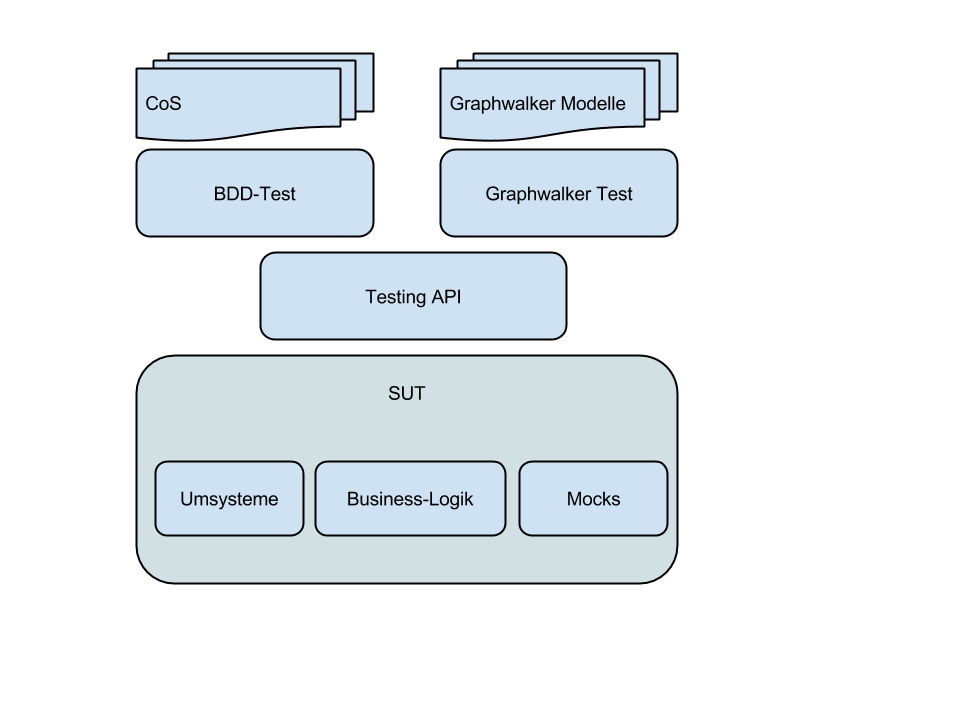
\includegraphics[width=1.0\textwidth]{figures/Testarchitektur-MBT-BDD-COS.png}
  \caption{Testarchitektur mit Behavior Driven Development und Model Based Testing Ansätzen}
  \label{fig:testarchitektur}
\end{figure}

\section{Aufbau der Teststufen}
Im Sinne von \Gls{Test-First} und einer hohen Priorisierung von Unit-Tests soll der Fokus des Testings auf drei Arten von Tests liegen:

\begin{itemize}
\item Eine breite Basis von Unit-Tests mit hoher Abdeckung
\item Modellbasierte Systemtests auf mehreren Ebenen mit direkter Verbindung zu Anforderungen/Changes
\item Manuelle System- und Abnahmetests
\end{itemize}

In Anlehung an Linz \cite{linz_testing_2014} soll die Komponententestebene in Scrum-Projekten am breitesten sein (siehe Abbildung \ref{fig:pyramide}).

\begin{figure}[h] 
  \centering
     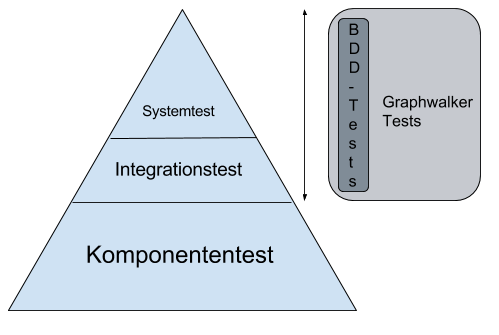
\includegraphics[width=1.0\textwidth]{figures/pyramide_mbt_bdd.png}
  \caption{Softwaretestpyramide und Einordnung der Teststrategie}
  \label{fig:pyramide}
\end{figure}

Dies erscheint mit Hinblick auf die vielen kurzen Iterationen, die das Softwaresystem stark verändern, auch logisch. Komponententests lassen sich, weil sie am entwicklungsnächsten sind, auch am schnellsten modifizieren. Obwohl Komponententests einzelne Komponenten in Isolation testen, müssen sie zumindest eine verlässliche Aussage treffen können, dass ebenjene Komponente ordnungsgemäß operiert. Diese Aussage wird möglich durch eine hohe Codeüberdeckung in Verbindung mit sorgfältig designten Testfällen. Auch auf Komponententestebene gelten Best-Practices und Methodiken für hochqualitative Testfälle, wie sie Spillner und Linz beschreiben \cite{spillner_software_2014}.\\
Die Besonderheit dieser hier vorgestellten Teststrategie liegt im Einsatz eines \Gls{BDT} \cite{chelimsky_rspec_2010} Frameworks und einer Testing-API. Es existieren einige frei erhältliche \Gls{BDT} Frameworks für viele gängige Programmiersprachen\footnote{Im Java-Umfeld bekannt sind die Frameworks \textit{jBehave} \url{http://jbehave.org/} und \textit{cucumber} \url{https://cucumber.io/}}. In der Fallstudie wurde aber eine Eigenentwicklung als \Gls{POC} gemacht (siehe Abschnitt \ref{sec:bdd} für eine Erläuterung). Die erwähnte Testing-API (siehe Abschnitt \ref{sec:testing_api}) bietet Schnittstellen zu Programmlogik und angebundenen Systemen.\\
Im Sinne dieser Arbeit steht der modellbasierte Anteil der Teststrategie im Mittelpunkt. Es soll aber erwähnt sein, dass keine zwei Softwareprojekte gleich sind und sich die Gewichtungen der Testmethodiken im Detail unterscheiden \textit{sollten}! Der modellbasierte Anteil basiert technisch ausschließlich auf quelloffenen Werkzeugen. Graphwalker (die Funktionsweise des Graphwalker-Frameworks wird in Abschnitt \ref{sec:graphwalker} erklärt) funktioniert als Testtreiber der das \Gls{SUT} systematisch durchläuft. Welche bzw. welche Art von Schnittstellen in das \Gls{SUT} greifen und es bedienen bleibt völlig offen und muss an die eigenen Bedürfnisse angepasst werden. Bei Applikationen mit GUI (oder wenn über die GUI \textit{End-to-End} Tests gemacht werden sollen) kann unter anderem Selenium\footnote{Webseite des Selenium-Projekts \url{http://www.seleniumhq.org/}} eingesetzt werden. Tests auf Schnittstellenebene können durch SoapUI\footnote{Offizielle Webseite von SoapUI \url{http://www.soapui.org/}} oder REST-assured\footnote{Code-Repository von REST-assured \url{https://code.google.com/p/rest-assured/}} angetrieben werden. Auch mächtigere proprietäre Werkzeuge können als Teil dieser Graphwalker-Teststrategie verwendet werden, sofern sie eine Schnittstelle zum Aufruf aus Java-Code besitzen und die Ergebnisse in beliebiger Form (bevorzugt als JUnit-Report) zurückliefern können (dieser Ansatz wurde in der Fallstudie nicht erprobt und wird deshalb nicht näher erläutert). Außerdem können Graphwalker-Modelle nicht nur Workflows darstellen, die auf GUI-Ebene ablaufen. Genauso vorstellbar sind Operationen die auf Schnittstellenebenen passieren (z.B. Operationen auf Datenbanken oder Web-Services). Bei solchen Tests macht es Sinn eine stabile Zwischenschicht, die Testing-API, einzubauen, die wiederrum auf die darunterliegenden Systeme zugreift. Der Aufwand zur Erstellung der API rechtfertigt sich, weil auch \Gls{BDT} Tests darüber in das \Gls{SUT} greifen.
Abbildung \ref{fig:pyramide} stellt dar, über welche Ebenen sich Tests mit \Gls{BDD} und Graphwalker erstrecken können.\\
Zuletzt bleiben aber auch manuelle Tests ein wichtiger Bestandteil der Teststrategie. Einerseits sind das Abnahmetests bei Neuentwicklungen beziehungsweise bei modifizierten Teilen des Systems und andererseits auch Regressionstests, die geschäftskritische Teile des Systems überwachen.

%%%%%%%%%%%%%%%%%%%%%%%%%%%%%%%%%%%%%%%%%%%%%%%%%%%%%%%%
\section{Details der Teststrategie und Architektur}
\label{sec:details}
%%%%%%%%%%%%%%%%%%%%%%%%%%%%%%%%%%%%%%%%%%%%%%%%%%%%%%%%


\subsection{Behavior Driven Testing Framework - FluentCoS}
\label{sec:fluent_cos}
In der Fallstudie hat sich gezeigt, dass die erwähnten \Gls{COS}-Tabellen (siehe Abschnitt \ref{sec:fallstudie}) schon recht genau \Gls{BDD}-Anforderungen entsprechen. Auch sie beschreiben, ausgehend von einem Ausgangszustand, welche Paramater zu einem bestimmten Endzustand führen sollen. Es lag also nahe diesen Ansatz zu verfolgen, bestehende Vorgehensweisen nicht grundlegend zu verändern und gleichzeitig bessere Spezifikationen zu schaffen. Außerdem bestand in der Fallstudie der Wunsch nach mehr automatischen Regressionstests, die genau jene \Gls{COS} prüfen. Mehrere Problemfelder wurden identifiziert, die mit dem Einsatz von \Gls{BDT} adressiert werden sollten:

\begin{itemize}
\item \textbf{Präzisierung der Spezifikation.} Spezifikationen in Prosatext und Fachjargon bieten ein hohes Potenzial für Missverständnisse und Ungenauigkeiten. Ein gemeinsames Vokabular und eine universell verständliche Syntax, um diese Spezifikationen festzuhalten, ist nötig.
\item \textbf{Spezifikationen müssen über lange Zeit überschaubar und prüfbar bleiben.} \Gls{COS} bleiben über viele Iterationen hinweg gültig. Es kommt aber immer wieder vor, dass sie direkt angepasst werden oder von anderen Weiterentwicklungen betroffen sind und geändert werden müssen. Die von den Fachbereichen verwendeten Storybooks lassen sich zwar versionieren (mittels bekannter Dokumenten-/Codeversionierungswerkzeuge) aber durch die schiere Größe dieser Dokumente ist es unmöglich festzustellen welche \Gls{COS} noch befriedigt sind und welche verletzt wurden. Es muss eine Form gefunden werden um \Gls{COS} kompakt, versionierbar und für alle an der Entwicklung Beteiligten verständlich, darstellen zu können.
\item \textbf{Einfache und nachhaltige Automatisierbarkeit der Regressionstests.} Aus den verfassten \Gls{COS} sollen, mit wenig Aufwand, automatisierte Regressionstests entstehen. Neben der einfachen Generierung dieser automatisierten Tests sollen vor allem die Aufwände für die Wartung niedrig gehalten werden.
\end{itemize}

Als \Gls{POC} wurde ein \Gls{BDT} Framework namens \textit{FluentCoS} entwickelt, das den Prinzipien von \Gls{BDD} treu ist. Dabei werden Tests in Java-Code verfasst, der sich sehr verständlich liest. Technisch werden Annotationen verwendet und das Framework stößt JUnit-Tests an. Implementierungsdetails finden sich im Anhangskapitel \ref{app:fluent}. Beispiel \ref{lst:bddcode} zeigt einen \Gls{BDD} Test. In den Kommentaren kann die \Gls{COS} als Prosa-Text erklärt werden. Dies entspricht der Anwendung in der \Gls{BDT} Vorlage aus Abschnitt \ref{sec:bdd}. Der Methodenname entspricht einer eindeutigen Identifizierung für die \Gls{COS}. Zentral sind die klar verständlichen Aufrufe an \textit{given}, \textit{when} und \textit{then}. Hier wird die Parallele zum fachlichen Anforderungsformat `Als Rolle fordere ich etwas und gewinne dadurch Nutzen' gezogen. Jeweils das zweite Argument innerhalb dieser Aufrufe entspricht einer Methode der Testing API (siehe Abschnitt \ref{sec:testing_api})

\begin{lstlisting}[caption={Beispielhaftes Codestück eines \Gls{BDD} Tests},label=lst:bddcode]

/**
 * Es muss fachlich sichergestellt sein, dass ...
 * Lorem Ipsum
 */
@Test
public final void cos_1_Hierarchische_Auflistung_und_Bezeichnung_des_Default_Teilvermoegens_Kontovermoegen() {
		given("Kunde XY fuer Beratung ausgewaehlt", selectCustomer("Peter Mueller"))
			.and("Kunde XY besitzt Produkte des TV's 'Kontovermoegen'", initCustomerAssets())
		.when("Berater fuer Kunde XY den Menuepunkt 'Anlegen Finfox' anklickt", clickMenu())
		.then("Wird das TV 'Kontovermoegen' an erster Stelle gezeigt", assertAccountFirst())
			.and("Der Titel des TV beinhaltet eine eindeutige Nummer", assertUniquePortfolioId())
			.and("Den TV-Typ 'Kontovermoegen'", nop());
}
\end{lstlisting}

Die eindeutige Identifikation als Methodennamen stellt sicher, dass eine unverwechselbare Parallele zwischen schriftlich festgehaltenen \Gls{COS} und automatisiertem Test hergestellt werden kann. Der Kommentarbereich kann zusätzlich verwendet werden, um auf Eigenheiten dieser \Gls{COS} einzugehen. Im Inneren der Methode werden dann Aufrufe mit der Struktur \textit{given} \textit{when} \textit{then} gemacht. Diese \Gls{BDD} Testfälle sind gut lesbar und lassen sich ohne weiteren Transformationen ausführen.\\
Bestehende Frameworks nutzen teilweise eine sogenannte \textit{Cleartext}-Syntax um den Testfall zu definieren. Natürlich handelt es sich aber nicht um natürlichsprachliches Englisch. Auch diese Syntax muss erlernt werden und wird in einem weiteren Schritt in JUnit-Code übersetzt. Wenn nun nicht-technische Domänenexperten in das Schreiben dieser BDD-Testfälle eingebunden werden sollen müssen sie sich jedenfalls eine neue Syntax aneignen. Bei der Cleartext-Variante wird ein weiterer, potenziell fehleranfälliger, Schritt nötig. Deshalb verzichtet FluentCoS auf diesen Zwischenschritt und arbeitet von Anfang an mit Java-Syntax.\\
Wenn das nicht-technisches Personal weiterhin nicht eingebunden werden soll, und daher die \Gls{COS} in Prosatext vorliegen, hat sich in der Fallstudie gezeigt, dass Entwickler es bevorzugen eine Programmiersprache für \Gls{BDD} Tests einzusetzen. Java-Entwickler sind allenfalls mit JUnit vertraut. Dies macht eine Cleartext-Syntax ebenfalls unnötig und spricht für die direkte Verfassung der \Gls{BDD} Testfälle in Java Code.\\
Denkbar wäre auch eine Teilung der Verfassung dieser \Gls{COS}. Da Fachbereiche und Entwickler gleichermaßen Zugriff auf die Versionsverwaltung haben, könnten die Fachbereiche die Klassen und Methoden anlegen. Die von ihnen identifizierten \Gls{COS} tragen sie ein. Das heißt sie erstellen eine Methode für jede \Gls{COS}. Sie verfassen jeweils das erste Argument der \textit{given} \textit{when} \textit{then} Aufrufe. Dabei handelt es sich tatsächlich um natürlichsprachliches Deutsch oder Englisch. Diese Dateien werden nun versioniert und den Entwicklern zugänglich gemacht. Die Entwickler, welche genaue Kenntnisse über die Testing API bzw. das \Gls{SUT} haben, tragen das zweite Argument ein. Meist ein Aufruf an die Testing API. Im weniger einfachen Fall muss ein \Gls{COS} umstrukturiert werden oder die Testing API muss erweitert werden.\\
Bei der Einführung dieser Methode sollte in kurzer Zeit eine komplette Umstellung auf als \Gls{BDT}-Testfall definierte \Gls{COS} erfolgen. Wenn Anforderungen in mehreren Formaten und an verschiedenen Stellen liegen führt dies zu Unklarheiten, Frustration (durch erhöhte Suchaufwände) und in weiterer Folge zu einem Abfall der Qualität. Dies hat sich in der Fallstudie gezeigt. Durch die starke Koppelung mit automatisierten Tests werden Anforderungen zwingendermaßen präziser. Damit wird auch Anforderung 1 (siehe Abschnitt \ref{sec:anforderungen_teststrategie}) erfüllt. Außerdem sind \Gls{COS} in Code-Form von Natur aus sehr kompakt. Für alle Beteiligten ist schneller greifbar welche \Gls{COS} bestehen.\\
Gleichzeitig bleiben gewisse Probleme bestehen: Obwohl \Gls{COS} nun direkt an automatisierte Regressionstests gekoppelt sind ist nicht garantiert, dass bei der Neueinführung eines Features, welches eine \Gls{COS} betrifft, sofort Alarm geschlagen wird. Wünschenswerterweise schlägt der dazugehörige Testfall zwar fehl, aber trotz aller Genauigkeit prüfen \Gls{COS} nur wenige Konstellationen. Dieses Problem adressiert die kombinierte Nutzung von \Gls{BDT} und \Gls{MBT} (siehe Abschnitt \ref{sec:mbt_bdt}).

\subsection{Testing API}
\label{sec:testing_api}

Konzeptuell ist die Testing API eine Schicht zwischen den Tests und dem \Gls{SUT} (siehe Abbildung \ref{fig:testarchitektur}). Konkret rufen die \Gls{BDT} Tests und die Methoden in den Graphwalker-Klassen die Schnittstelle auf, um Operationen am \Gls{SUT} auszuführen. Im Sinne des vereinheitlichten Vokabulars von \Gls{BDD} ist diese Schicht eine uniforme Sicht auf das \Gls{SUT}.\\
Das Design der Testing API soll wohlüberlegt sein und die folgenden Anforderungen erfüllen:

\begin{enumerate}
\item \textbf{Design for maintenance (Entwurf mit Fokus auf Wartung)}: Da das zugrundeliegende \Gls{SUT} ständigen Änderungen ausgesetzt ist, wird auch die darauf zugreifende Schnittstelle angepasst werden müssen. Die Architektur dieser API muss auf einfache Wartbarkeit und langfristiges Bestehen ausgelegt sein.
\item \textbf{Abstraktionslevel}: Die Testing API soll ausdrücklich keine Unit-Testing API sein. Die API muss auf den richtigen Level abstrahiert werden, um sinnvoll einsetzbar zu sein. Einerseits muss die Bedienung des \Gls{SUT} feingranular erfolgen können. Andererseits muss es trotzdem möglich sein die kundensichtbaren Aktionen, ohne Kenntnisse der Interna, auslösen zu können. \citeauthor{tyler_black-box_2004} sprechen von einer \textit{Grey-Box Sicht} \cite{tyler_black-box_2004}.
\item \textbf{Niedrige Komplexität}: Jede Schicht zwischen Test und \Gls{SUT} ist eine potenzielle Fehlerquelle. Die Testing API darf nicht zu einem eigenen Software-Projekt ausarten. Wenn Testfälle ein Fehlverhalten melden muss so schnell wie möglich und mit wenig Aufwand feststellbar sein welche Komponente es verursacht hat. Wenn die Schnittstelle undurchsichtig ist müssen Aufwände betrieben werden, um das korrekte Verhalten dieser zu garantieren.
\end{enumerate}

Neben den in der Softwareentwicklung bekannten Vorgehensweisen um die  Wartbarkeit zu erhöhen erfordert Anforderung 1 keine weiteren speziellen Kenntnisse. Trotzdem ist diese Anforderung nicht leicht zu erfüllen, vor allem wenn sich die Struktur der Business-Logik des \Gls{SUT} verändert. Änderungen in der Schnittstelle dürfen also nicht immer einfach angepasst werden. Die darauf aufbauenden Testfälle könnten möglicherweise brechen oder, noch schlimmer, weiterhin funktionieren aber falsche Testergebnisse liefern. Änderungen müssen sorgfältig nach außen kommuniziert werden und es muss auch in Betracht gezogen werden, dass Testfälle fehlschlagen wenn Methoden- oder Klassennamen umbenannt werden.\\
%Das heißt, Änderungen müssen wohldefiniert nach außen kommuniziert werden und gegebenenfalls darf nicht davor zurückgescheut werden Testfälle durch Umbenennungen von Methoden- oder Klassennamen zu brechen.\\ Satz wirkt so als wäre er 1:1 aus dem engischen Übersetzt
Diese Überlegung führt zu einem weiteren Knackpunkt im Design der gesamten Teststrategie: Um Parteien, die keinen Zugriff auf Quellcode haben, in die Erstellung der Testfälle miteinzubeziehen, müssem sie über die Operationen, die die Testing API bereitstellt, bescheid wissen. Ist dies nicht der Fall, können sie nur rudimentäre \Gls{BDT} Tests schreiben, die ohne Zutun der Entwickler nicht lauffähig sind. Es ist also ein Plan von Nöten wie dieser Katalog von Methoden, die die Testing API anbietet, propagiert wird. Dies muss jedenfalls automatisiert erfolgen um weitere Aufwände mit der Synchronisierung bei Änderungen zu vermeiden. Denkbar ist die Nutzung automatischer Generierung von Dokumentation aus Code-Kommentaren\footnote{Im Java-Umfeld ist das Werkzeug \textit{JavaDoc} weitverbreitet, welches aus Kommentaren einer API Dokumentation in Form von HTML, inklusive Navigation, generieren kann \url{http://www.oracle.com/technetwork/articles/java/index-jsp-135444.html}}. Diese Dokumentationsdateien sind dadurch eng an den Code der Testing API gekoppelt und versioniert. Außerdem können so nicht nur die Namen der Methoden sondern auch fachliche und technische Erklärungen angehängt werden.\\
Anforderung 3 betrifft die Umfänge und Komplexität der Schnittstelle. Um mit der API die richtige Abstraktion aus Anforderung 2 treffen zu können, ist es unumgänglich einige Werte zu modifizieren und mehrere Aufrufe zu machen. Auch die Entwicklung dieser API soll in die agile Entwicklung inklusive \Glspl{Review} und Komponententests einfließen. Trotzdem ist es von höchster Priorität sich zugunsten niedriger Komplexität zu entscheiden, auch wenn in manchen Fällen Anforderung 2 kompromitiert wird. Zu hohe Aufwände für das Testen oder die Verifikation der Testing API würden die Zeitersparnisse der neuen Teststrategie zunichte machen.

\subsection{Modellbasierte Tests mit Graphwalker}
\label{sec:mbt_results}
Die Fallstudie hat gezeigt, dass die Diversität der zu testenden Gesichtspunkte des \Gls{SUT} zu hoch ist, um einen allumfassenden Ansatz einzusetzen. Dieser Schluss lässt sich mit Sicherheit auf eine große Anzahl von Softwareprojekten übertragen. Selten lassen sich alle wertgenerierenden Aspekte mit einer Art von Tests prüfen. Auch die hohe Anzahl von beteiligten Personen, ob technisch oder fachlich, suggeriert, dass nicht alle dieselben Fähigkeiten und Vorlieben für eine Testmethode an den Tag legen.\\
Diese Beobachtungen legen nahe, ein schlankes und flexibles Werkzeug für den modellbasierten Teil der Teststrategie einzusetzen. Repräsentativ für große agile Softwareprojekte ergaben sich weitere Anforderungen an Werkzeug und Umgebung der modellbasierten Tests:

\begin{itemize} 
\item\textbf{Eignung der Feststellung} Es sollte mit wenig Aufwänden möglichen sein, die Eignung des Werkzeugs für das Testing des \Gls{SUT} festzustellen. Dies setzt erstens voraus, dass vollwertige Testversionen zur Verfügung gestellt werden. Zweitens muss die Funktionsweise, wie das Werkzeug im Hintergrund agiert, dokumentiert und einsehbar sein. Dies ist bei den wenigsten Werkzeugen der Fall. Graphwalker, ist durch seine Quelloffenheit eine erfreuliche Ausnahme.
\item \textbf{Flexibilität des Modellformats} Vergleichbar mit der Sprache, in der die Skripts eines skriptbasierten Werkzeugs vorliegen müssen, sind Modellformate für \Gls{MBT} Werkzeuge strikt vorgegeben. Wie effektiv ein \Gls{SUT} getestet werden kann hängt massiv von der Mächtigkeit des Modellformats ab.
\item \textbf{Verständlichkeit des Modellformats} Das Modellformat an sich, aber auch die Präsentation dessen muss verständlich sein.
\end{itemize}

Modellbasiertes Testen kann immer noch als Randerscheinung im Softwaretesten angesehen werden. Die Auswahl an Werkzeugen ist deshalb überschaubar. Gerade deswegen ist es schwer diese Werkzeuge miteinander zu vergleichen. Sie unterscheiden sich in ihrer Art erheblich. Manche Hersteller entwerfen ihre Werkzeuge als Komplettlösung für das Testen auf mehreren Teststufen. Dieser Komplettlösungsansatz erschwert eine Einführung in ein bestehendes Softwareprojekt. Eine Prüfung auf Eignung muss umso umfangreicher erfolgen. Nach einer Einführung kann schwerer auf eine andere Teststrategie umgeschwenkt werden.\\
Aus Sicht des Entwicklers ist es wünschenswert die interne Vorgehensweise dieser Werkzeuge zu kennen. Dazu zählen die Möglichkeiten wie das \Gls{SUT} modelliert werden kann aber auch entscheidende Details wie das Testdatenmanagement und die Integrationsfähigkeit in die bestehende Umgebung, da meist auf existierende Infrastrukturen Rücksicht genommen werden muss. Dementsprechend sollte nur mit Zugriff auf Dokumentation und Testversionen herausgefunden werden welche Fähigkeiten die Werkzeuge bieten und ob sie sich grundsätzlich in das Projekt integrieren lassen.\\
Wie auch im Abschnitt \ref{sec:notations} theoretisch beschrieben und im Diskussionsabschnitt \ref{sec:discussion_format} angesprochen, bestehen massive Unterschiede zwischen Werkzeugen und deren Modellformaten. Einen weitverbreiteten Standard gibt es nicht und deshalb stellt sich die Frage des Modellformats bei jeder Einführung von \Gls{MBT} in einem Projekt. Auch in der Fallstudie dieser Arbeit war dies der Fall. Eine Eigenentwicklung ist aus mehreren Gründen nicht ratsam. Erstens ist der Entwicklungsaufwand sehr hoch, da keines der evaluierten Werkzeuge die Möglichkeit bietet nur die Sprache selbst zu definieren. Neben formaler Definition der Sprache und Entwicklung eines Lexers und Parsers müsste also die gesamte restliche Infrastruktur entwickelt werden. Dazu zählt die Traversierungslogik, das Reporting und weitere Komponenten. Zweitens würden auch Eigenentwicklungen auf bekannte Modellierungssprachen setzen und könnten das Rad sozusagen nicht neu erfinden. Der Zugewinn an Funktionalität, den Entwicklungsaufwänden gegenübergestellt, wäre wahrscheinlich klein.\\


\subsubsection{Entscheidende Eigenschaften von Graphwalker}
Graphwalker funktioniert sehr gut als flexibles Grundgerüst für das modellbasierte Testen und kam in der Fallstudie aufgrund der folgenden Eigenschaften zum Einsatz:

\paragraph{Simples aber mächtiges Modellformat} Wie der Name schon sagt basiert das Modellformat von Graphwalker auf Graphen (siehe Abschnitt \ref{sec:graphwalker} zu Graphwalker). Die Entwickler von Graphwalker haben festgestellt, dass gerichtete Graphen ausreichend ausdrucksstark sind um Softwaresysteme zu testen \cite{_graphwalker_2015}. Notationen wie das UML Testing Profile (siehe Abschnitt \ref{sec:utp}) bieten eine Vielzahl von verschiedenen Elementen, welche die Modelle mächtiger aber gleichzeitig überladen wirken lassen. Die Semantik der Modelle ist ohne Einschulung kaum greifbar.\\
Graphwalker bietet trotzdem genug Funktionalität, um die Modelle handhabbar zu machen. Einerseits geht es um die Modularisierung des \Gls{SUT}. Bestimmte Funktionalitäten sind an verschiedenen Stellen im System immer wieder gefordert. Genau wie der zugrundeliegende Quellcode für diese Zwecke modularisiert worden ist, so soll auch das Modell des \Gls{SUT} modularisierbar sein. Graphwalker erlaubt daher die Aufteilung des Modells in mehrere Teile und die Markierung eines Knoten als \textit{Sprungknoten}. Von diesen Knoten aus kann bei der Traversierung in eine andere Modelldatei gesprungen werden. Dort wird die Traversierung fortgesetzt und, falls vorhanden, über einen weiteren \textit{Sprungknoten} zurückgekehrt.

\paragraph{Transparente Vorgehensweise} Das einfache Modellformat und die schnörkellose Präsentation des Werkzeugs, kombiniert mit Quelloffenheit und guter Dokumentation, lassen Graphwalker sehr transparent wirken. Nach der Modellierung können Fachbereiche als auch Entwickler schnell begreifen wie die Traversierung gemacht wird und welche Aktionen am \Gls{SUT} ausgeführt werden. Diese genaue Steuerung der Tests ist wichtig um überhaupt sinnvolle Testsuiten designen zu können. Bei der Modellierung des \Gls{SUT} müssen nuancierte Details unterscheidbar sein. Soll heißen, dass technisch versierte als auch weniger versierte Stakeholder verstehen was modelliert wurde. Es sei auf den Abschnitt \ref{sec:results_modellierung} hingewiesen, wo die Möglichkeiten zur Modellierung im Detail beschrieben werden.


%%%%%%%%%%%%%%%%%%%%%%%%%%%%%%%%%%%%%
\subsubsection{Möglichkeiten zur Modellierung - Arten von fachlichen Modellen}
\label{sec:results_modellierung}
%%%%%%%%%%%%%%%%%%%%%%%%%%%%%%%%%%%%
Nun werden die Möglichkeiten zur Modellierung eines mehrteiligen Workflows aus Kundensicht geschildert. Als laufendes Beispiel dient eine Internetanwendung aus der Fallstudie Raiffeisen\footnote{Alle Screenshots wurden am 28.07.2015 auf der öffentlich zugänglichen Seite \url{https://www.raiffeisen.ch/content/www/rch/de/privatkunden/hypotheken/wohneigentum-kaufen/wieviel-eigenheim-kann-ich-mir-leisten.html} gemacht.}. Dabei handelt es sich um einen Hypothekarrechner für Privatkunden.\\
Basierend auf mehreren Parametern (Kaufpreis, Eigenkapital, Jahreseinkommen) wird kalkuliert, ob eine Hypothek vergeben werden kann oder nicht (Tragbarkeit). Bei gegebener Tragbarkeit folgen vier Fragen, die auf die Risikobereitschaft des Kunden und das erwartete Zinsniveau abzielen. Sie haben das Ziel eine passende Kombination von Produkten vorzuschlagen. Abschließend kann ein Beratungstermin bei einer regionalen Niederlassung vereinbart werden.\\
Dieser Ablauf ist starr. Es macht also keinen Unterschied wie der Benutzer die vier Fragen beantwortet, die Sequenz bleibt immer dieselbe. Zur besseren Übersicht wird bei den folgenden Modellen nur die Vorwärts-Richtung modelliert. Um das Verhalten beim Klick auf die ``Zurück'' Schaltfläche zu modellieren, müssten einfach Kanten in die andere Richtung eingefügt werden.\\
Die Graphwalker Kommandozeilenapplikation generiert aus jedem Modell ein Java-Interface und aus jeder Kante sowie jedem Knoten eine Methode. Haben aber mehrere Knoten oder Kanten im Modell denselben Bezeichner, so wird im Interface nur eine entsprechende Methode generiert. Der Testentwickler muss bei der Modellierung also entscheiden, ob sich ein Knoten oder eine Kante so voneinander unterscheiden, dass verschiedene Code-Bausteine ausgeführt werden müssen. Wenn ja, müssen die betroffenen Elemente im Modell unterschiedliche Bezeichner erhalten.\\
Die gerade beschriebene Thematik ist eine der Hauptpraktiken um die Komplexität eines Modells zu reduzieren, denn eine niedrigere Anzahl an eindeutig identifizierbaren Elementen mindert die Anzahl an Codezeilen, die gewartet werden müssen. Die zweite Möglichkeit ein Modell übersichtlicher und gleichzeitig wiederverwendbar zu machen ist die Aufteilung in mehrere Modelle (also mehrere GraphML-Dateien) und die Definition von Sprungpunkten (diese Funktionsweise wird in Abschnitt \ref{sec:graphwalker_modularisierung} beschrieben).\\
Im Folgenden wird der oben beschriebene Ablauf (das \Gls{SUT}) auf zwei verschiedene Arten modelliert und die Vor- und Nachteile der jeweiligen Methode erläutert.


\paragraph{Workflow-Modellierung. Knoten: 10, Kanten: 17}
Diese Art der Modellierung ergibt das kleinste Modell (Zahl der Knoten und Kanten in Summe). Das \Gls{SUT} wird gewissermaßen als Blackbox gesehen, wobei aus der Modellierungssicht nicht klar ist welche Auswirkungen die Eingaben haben. An diesem Beispiel startet man also auf dem Knoten \texttt{v\_OnPage}, welcher die Startseite des \Gls{SUT} darstellt. Es werden drei numerischen Eingaben gemacht (dies passiert in der Kante \texttt{e\_EnterCredibility}). Nun folgt ein weiterer Klick in der Kante \linebreak \texttt{e\_ClickStartProposal}. Hier könnte das Modell nun verzweigen, da die erste der vier Fragen mit drei möglichen Antworten folgt. In der Workflow-Modellierung werden die drei Antwortmöglichkeiten durch die Kanten \texttt{e\_Planbare\_unwichtig}, \texttt{e\_Planbare\_wichtig} und \texttt{e\_Planbare\_sehrWichtig} dargestellt. In den entsprechenden \textbf{drei} Methoden dieser Kanten befinden sich die Aufrufe an Methoden, die die Schaltflächen anklicken. Alle Kanten führen aber wieder zu einem einzigen Knoten, der die nächste der vier Fragen darstellt.\\
In diesem Beispiel erfolgt eine entscheidende Ergebnisanzeige im letzten Arbeitsschritt \linebreak (\texttt{e\_finalProposal}). Dieses Ergebnis ist aber sehr wohl abhängig davon auf welchem Pfad das \Gls{SUT} durchlaufen wurde. Aus dem Modell ist dieser Pfad aber nicht ersichtlich. Die Komplexität dieser Rekonstruktion des Pfades befindet sich vollständig im Code und ist im Modell unsichtbar. Die Abbildung \ref{fig:modell_abstract} zeigt das Modell des erwähnten Workflows.\\
Aus Sicht der Wartungsfreundlichkeit kann keine generelle Aussage getroffen werden. Da das Modell aus wenigen Elementen besteht hält sich der Aufwand dort in Grenzen. Wieviel Aufwand in die Ändernugen im Code investiert werden muss ist davon abhängig wie die Rekonstruktion gelöst wurde und welche Struktur das \Gls{SUT} aufweist. Trotzdem ist diese Vorgehensweise eine valide Option, da die Komplexität des Modells sehr niedrig gehalten wird und dies die erhöhte Komplexität im Code rechtfertigen kann.

\begin{figure} 
  \centering
     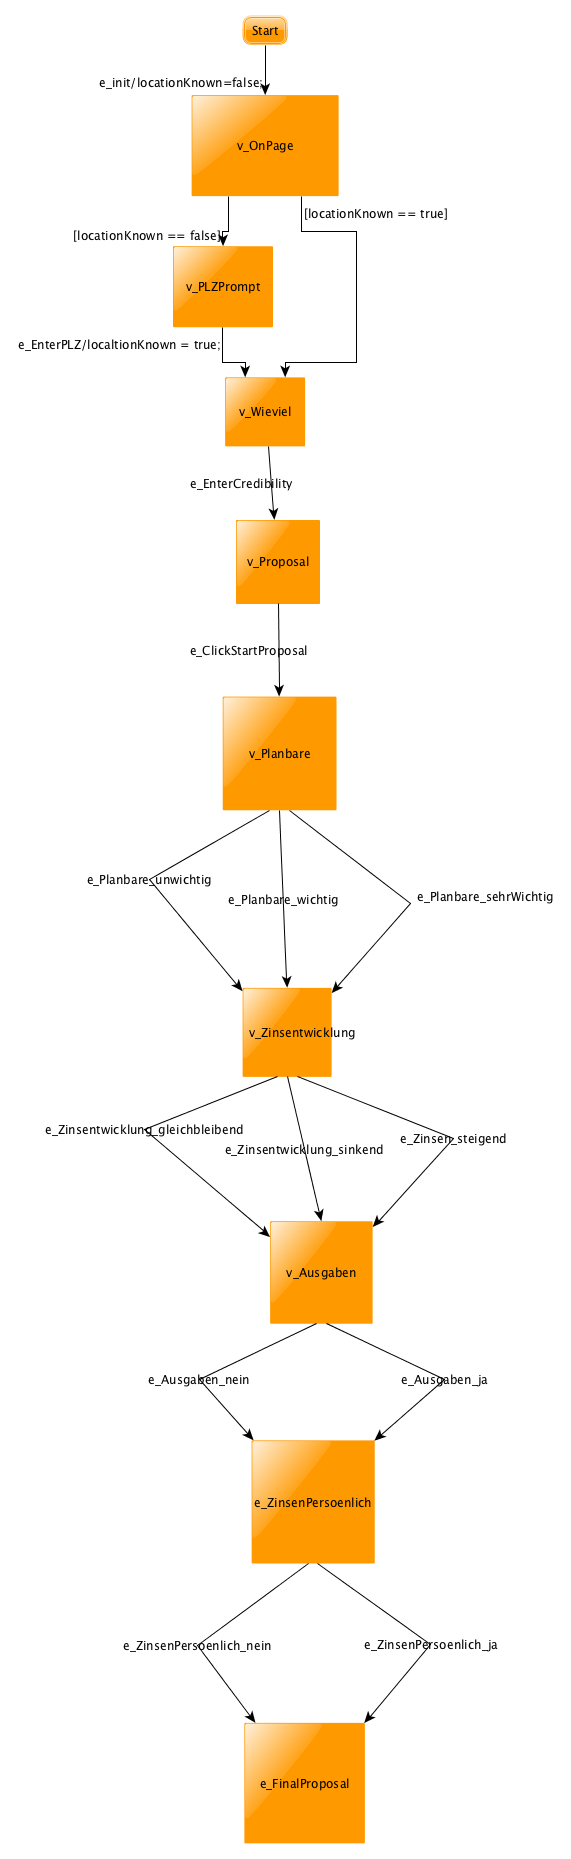
\includegraphics[width=0.45\textwidth]{figures/modell_abstract.png}
  \caption{Abstrakte Version eines Modells der Fallstudie}
  \label{fig:modell_abstract}
\end{figure}

\paragraph{Logik-Modellierung und Verfeinerung. Knoten: 72/51, Kanten: 72/66} Bei der Logik-Modellierung wird das System nicht mehr als reine Blackbox gesehen. Das Modell soll weiterhin eine Abstraktion des \Gls{SUT} sein aber der Detailgrad erhöht sich. Dies hat zur Folge, dass zwar mehr Knoten und Kanten erstellt werden müssen, die Komplexität im Code sich aber verringert. Erreicht wird dies durch die explizite Modellierung von Kanten und Knoten mit \textbf{identischen} Bezeichnern. In diesem Beispiel, wo nur der Endzustand \texttt{v\_finalProposal} einer detaillierten Prüfung unterzogen wird, erhalten nur die Knoten auf unterster Ebene eindeutige Bezeichner. Graphwalker generiert nun zwar 36 Methoden(entsprechend den 36 Knoten mit den Bezeichnern \texttt{v\_finalProposalXX}, die dem Knoten \texttt{v\_finalProposal} aus dem Workflow-Modell entsprechen, aber diese enthalten keinerlei Logik um den Pfad zu reproduzieren. In diesen Methoden befindet sich also nur ein Bruchteil der Logik die im letzten Knoten der Workflow-Modellierung zu finden ist. Durch die explizite Modellierung aller möglichen Pfade ist implizit gegeben wie das \Gls{SUT} traversiert wurde und welche Prüflogik angewandt werden muss. Die Abbildung \ref{fig:modell_komplex} zeigt die logisch modellierte Variante des Hypothekarrechners.

% \begin{figure}[h] 
%   \centering
%      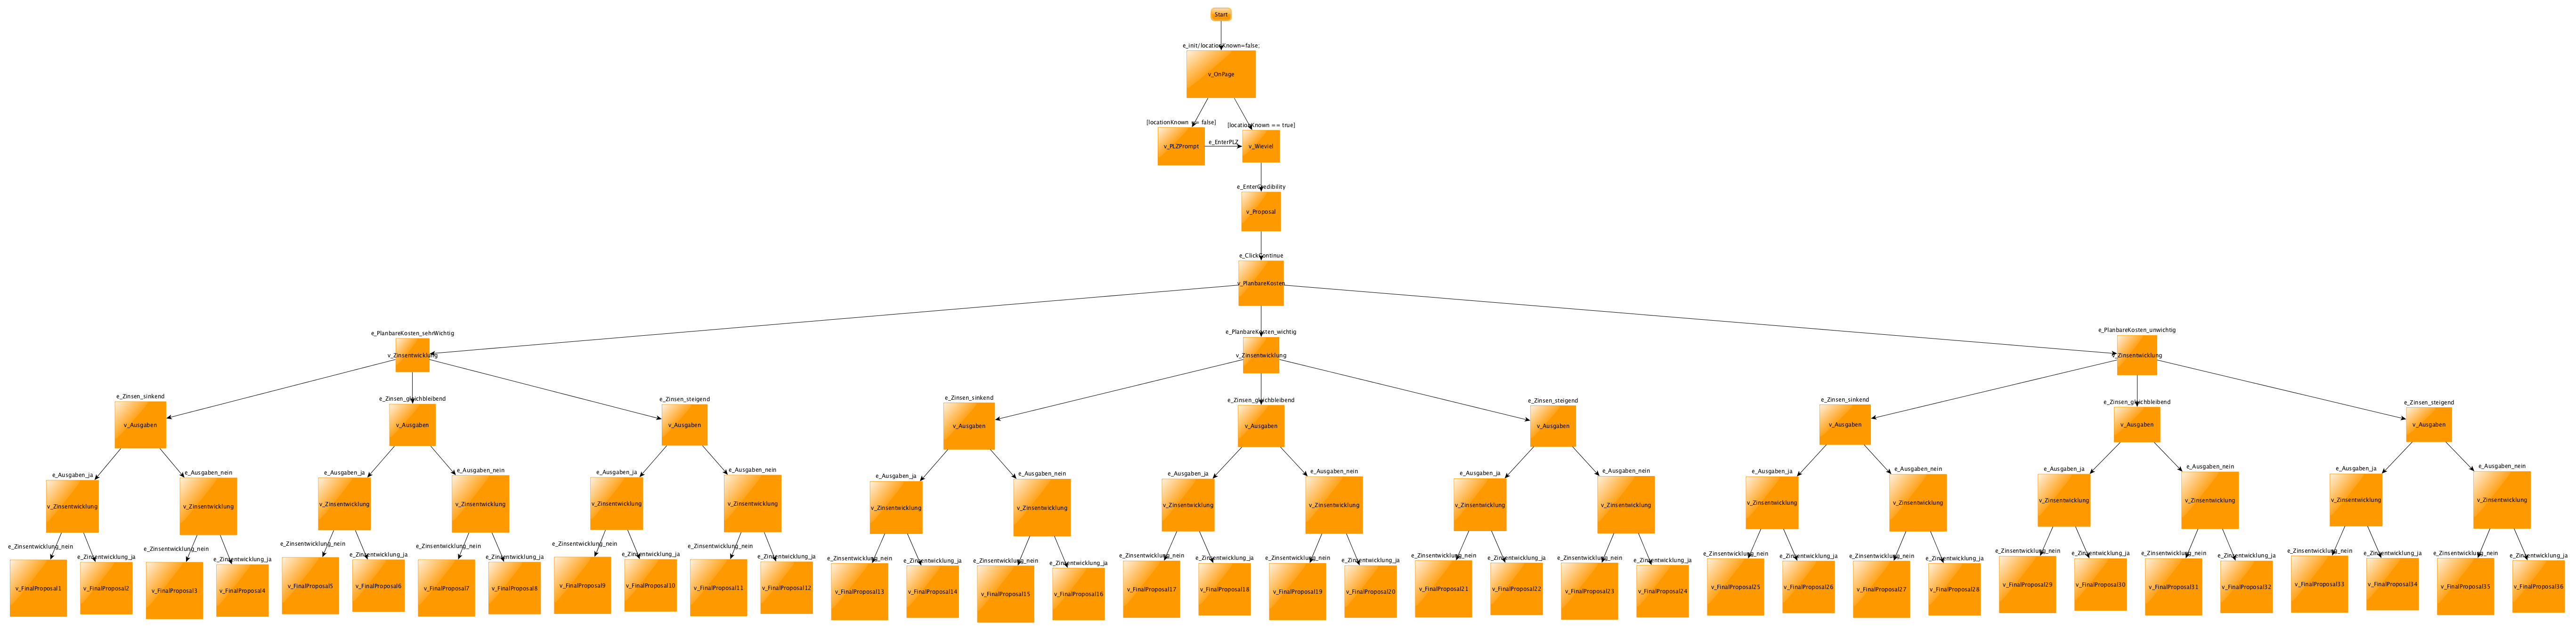
\includegraphics[width=1.5\textwidth, angle=90]{figures/modell_komplex.png}
%   \caption{Logisch modellierte Variante des Modells mit 72 Knoten und 72 Kanten.}
%   \label{fig:modell_komplex}
% \end{figure}

\begin{figure}[p] \begin{leftfullpage}
\hspace*{-2.5cm}
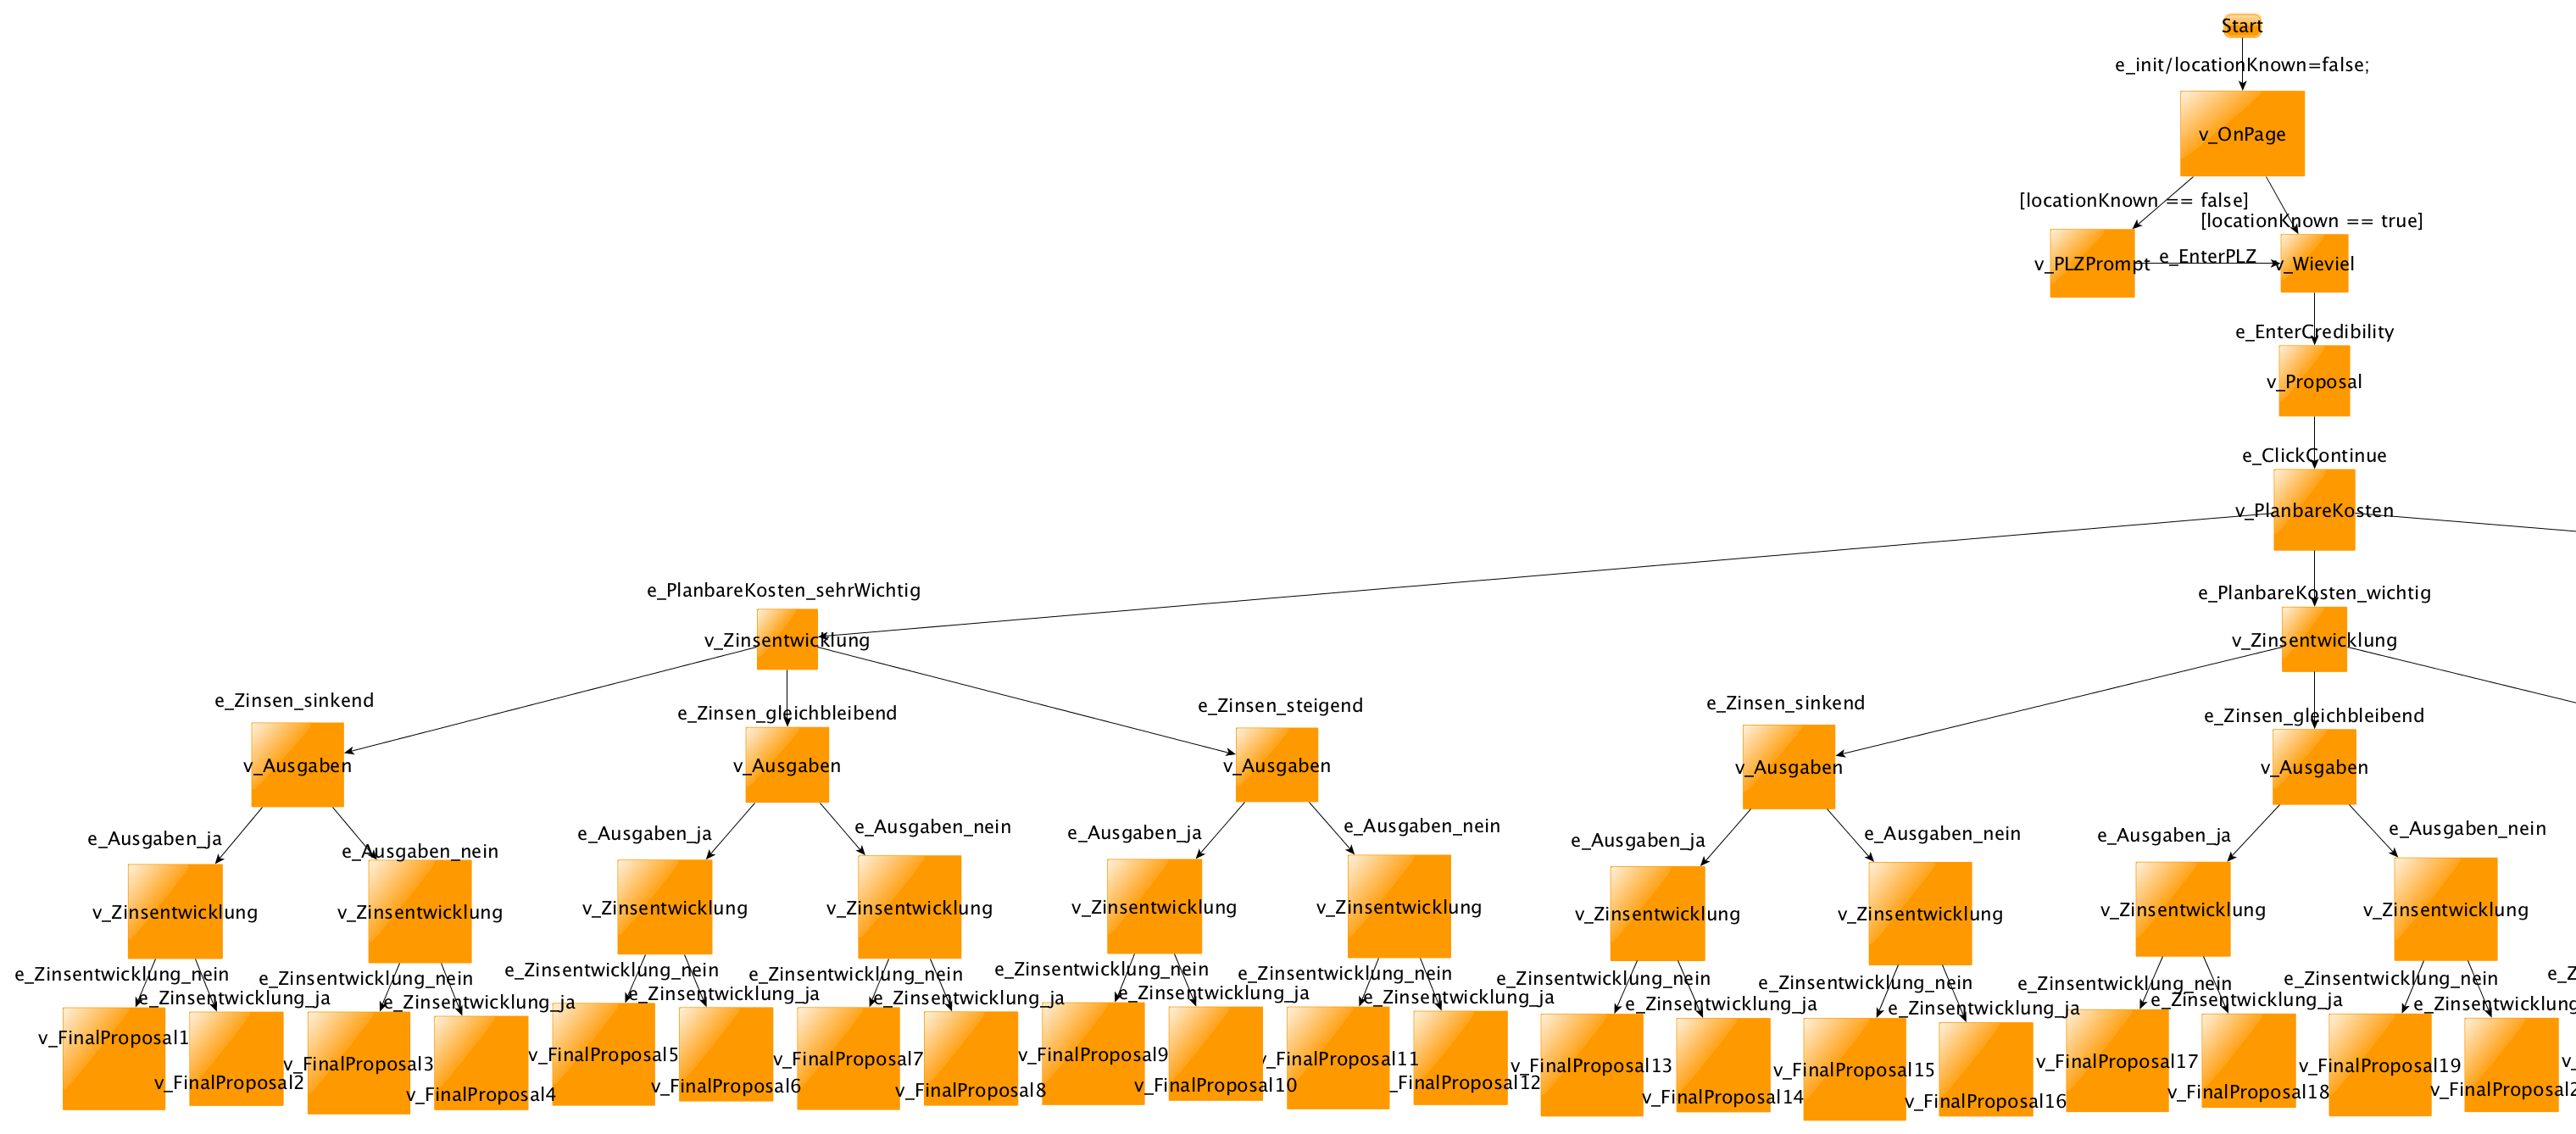
\includegraphics[width=1.2\textwidth]{figures/modell_komplex_left.png}
\caption{Logisch modellierte Variante des Modells mit 72 Knoten und 72 Kanten. Linke Seite.}
\label{fig:modell_komplex}
\end{leftfullpage} 
\end{figure} 
\begin{figure}[p] 
\begin{fullpage} 
\hspace*{-2.5cm}
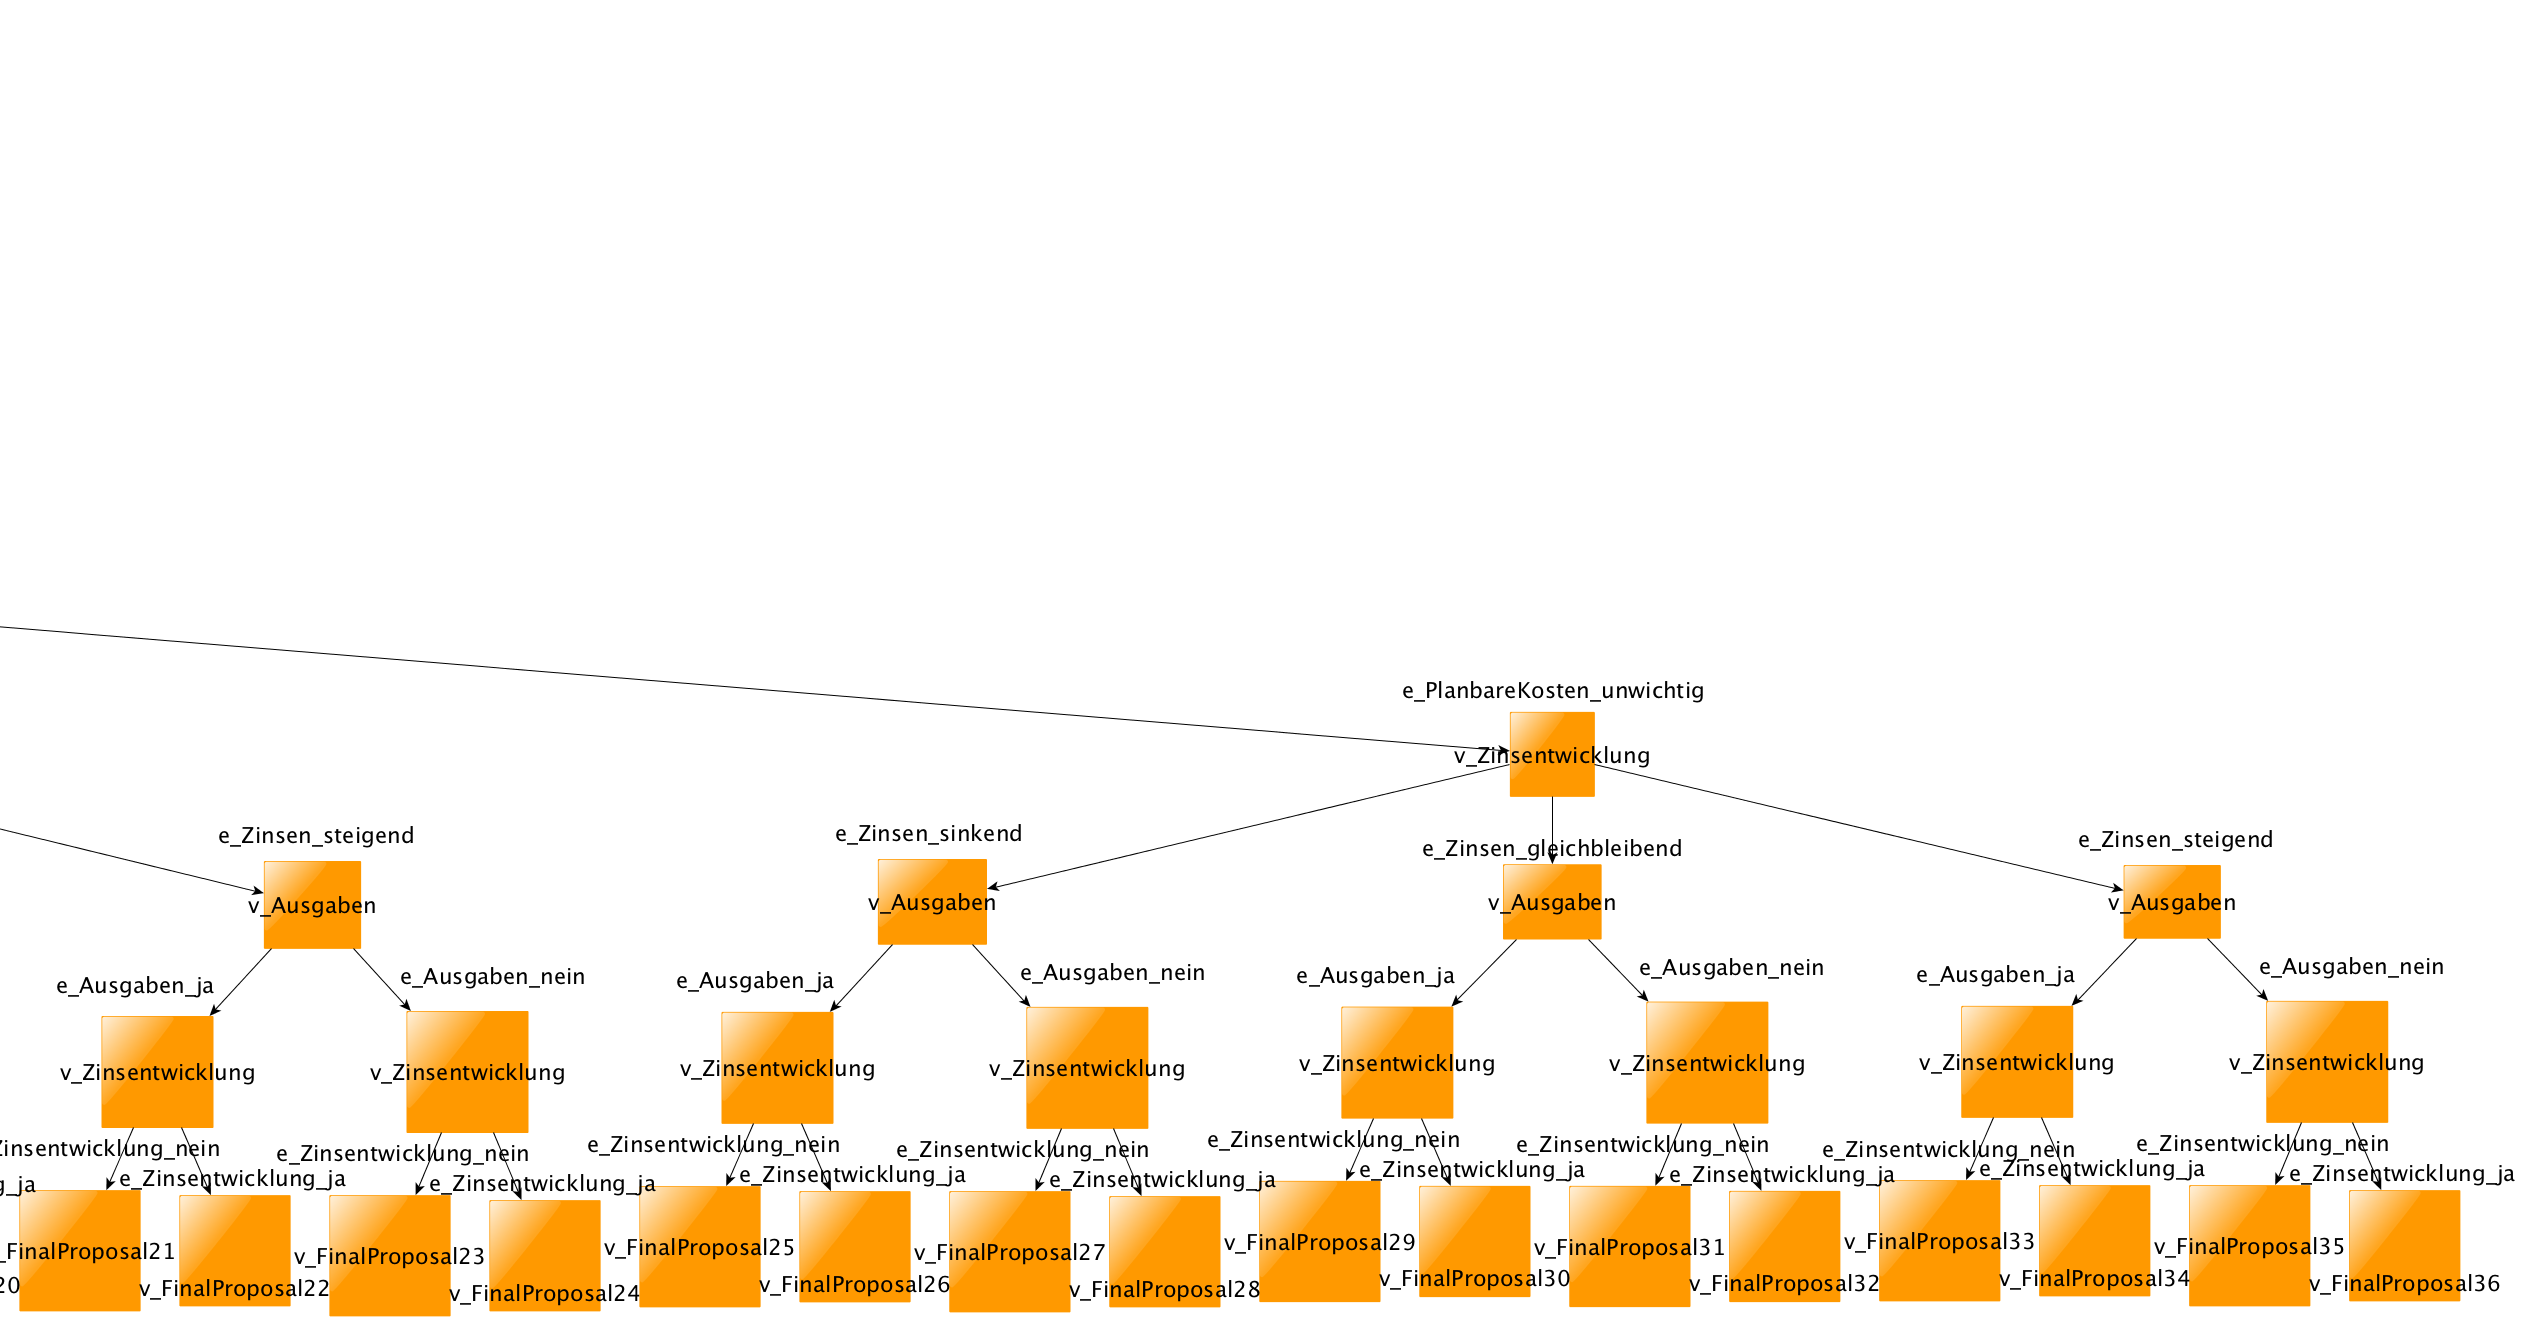
\includegraphics[width=1.2\textwidth]{figures/modell_komplex_right.png}
\caption{Logisch modellierte Variante des Modells mit 72 Knoten und 72 Kanten. Rechte Seite.}
\end{fullpage} \end{figure} 

Es fällt schnell auf, dass das Hinzufügen von nur wenigen Auswahlmöglichkeiten im Prinzip dasselbe aus dem \textit{Model Checking} bekannte Problem der kombinatorischen Zustandsexplosion aufwirft \cite{clarke_model_2012}. Verglichen mit den Ansätzen aus diesem Feld (wie \textit{Counterexample-guided abstraction refinement} \cite{clarke_counterexample-guided_2000}), bei denen eine Abstraktion verfeinert wird, geht man hier aus der anderen Richtung vor. Man betrachtet die Programmlogik auf Code-Ebene genauer und versucht Abstraktionen des komplexen Modells zu generieren. Bei numerischen Werten können zum Beispiel weniger Werte modelliert werden (Konzentration auf Grenz- und Extremwerte). Beim Beispiel des Hypothekarrechners stellte sich heraus, dass die zugrundeliegende Programmlogik gar keine 36 Ergebniskategorien erzeugen kann. Die beiden letzten der vier Fragen generieren also keine eigene Ergebniskategorie sondern \textit{schieben} das Ergebnis in eine der anderen Kategorien. Tatsächlich ergeben sich viel weniger Pfade als im ursprünglichen Modell und es bleiben nur 51 Knoten sowie 66 Kanten. Gezeigt wird diese vereinfachte Version des Modells in Abbildung \ref{fig:modell_logisch}. Gut zu sehen sind die Überschneidungen auf zweitletzter Ebene, die zu deutlich weniger Endzuständen und damit zu weniger Code führen.\\
Durch eine verstärkte Whitebox-Ansicht muss der Modellierer also versuchen die Zustände und Übergänge im Modell zu verringern.

\todo[color=blue]{Nur die zweite doppelseitige Grafik hat die vergrößerte Schriftgröße. Die andere doppelseitige Grafik wird noch nachgereicht.}

% \begin{figure}[h] 
%   \centering
%      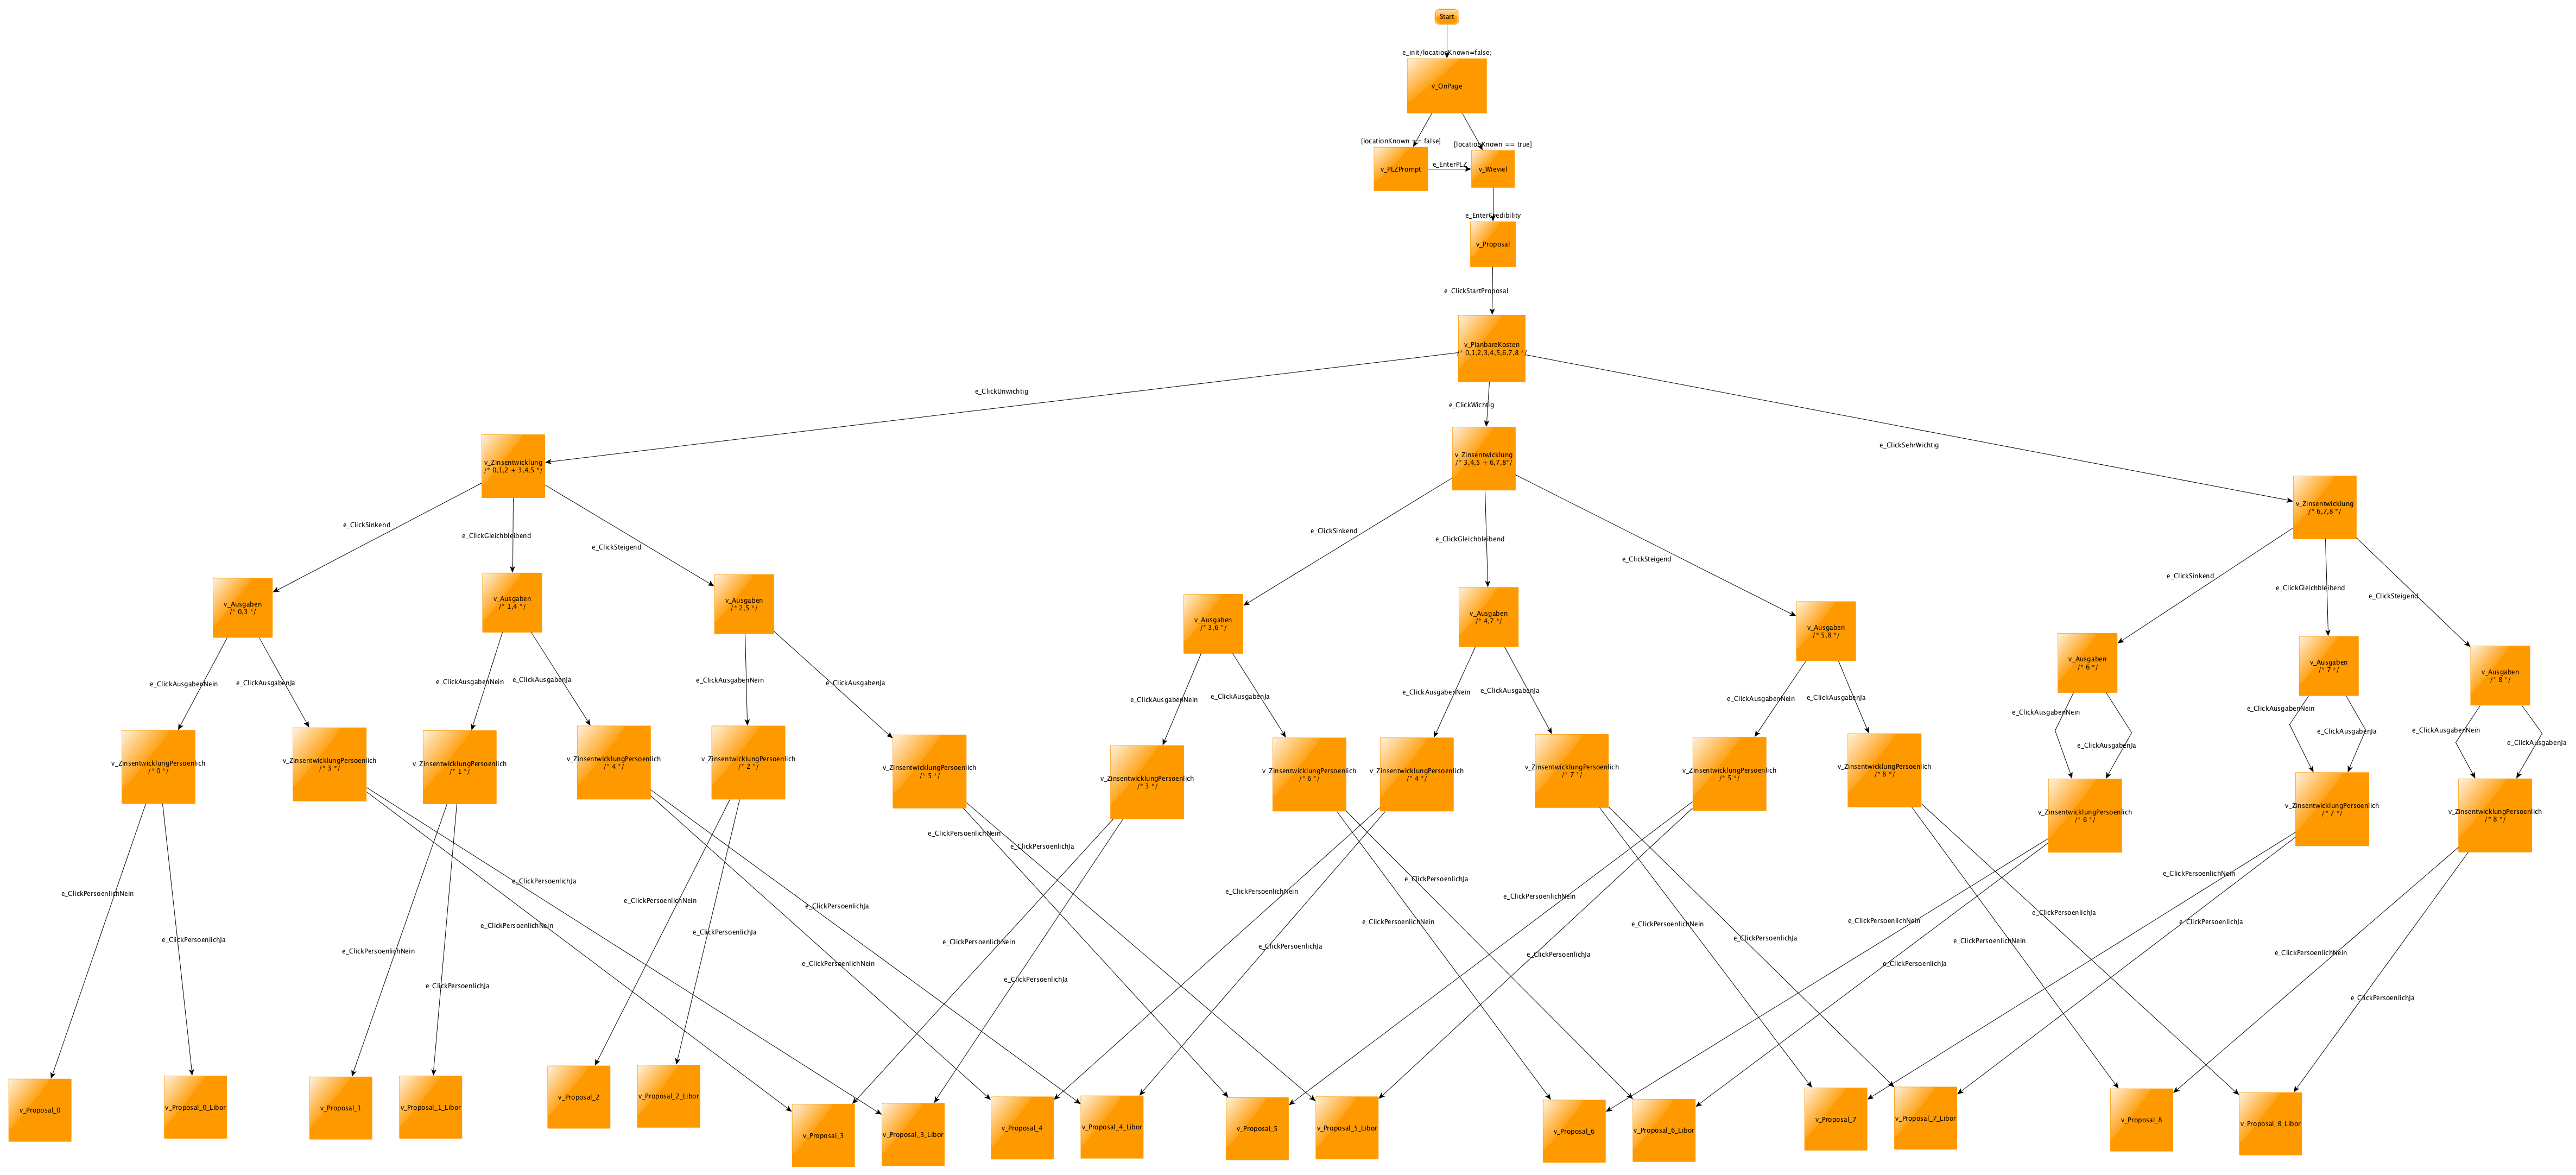
\includegraphics[width=1.5\textwidth, angle=90]{figures/modell_logisch.png}
%   \caption{Ausgehend von der Logik-Modellierung wurde hier die Logik im Quellcode betrachtet.}
%   \label{fig:modell_logisch}
% \end{figure}

\begin{figure}[p] \begin{leftfullpage}
\hspace*{-2.5cm}
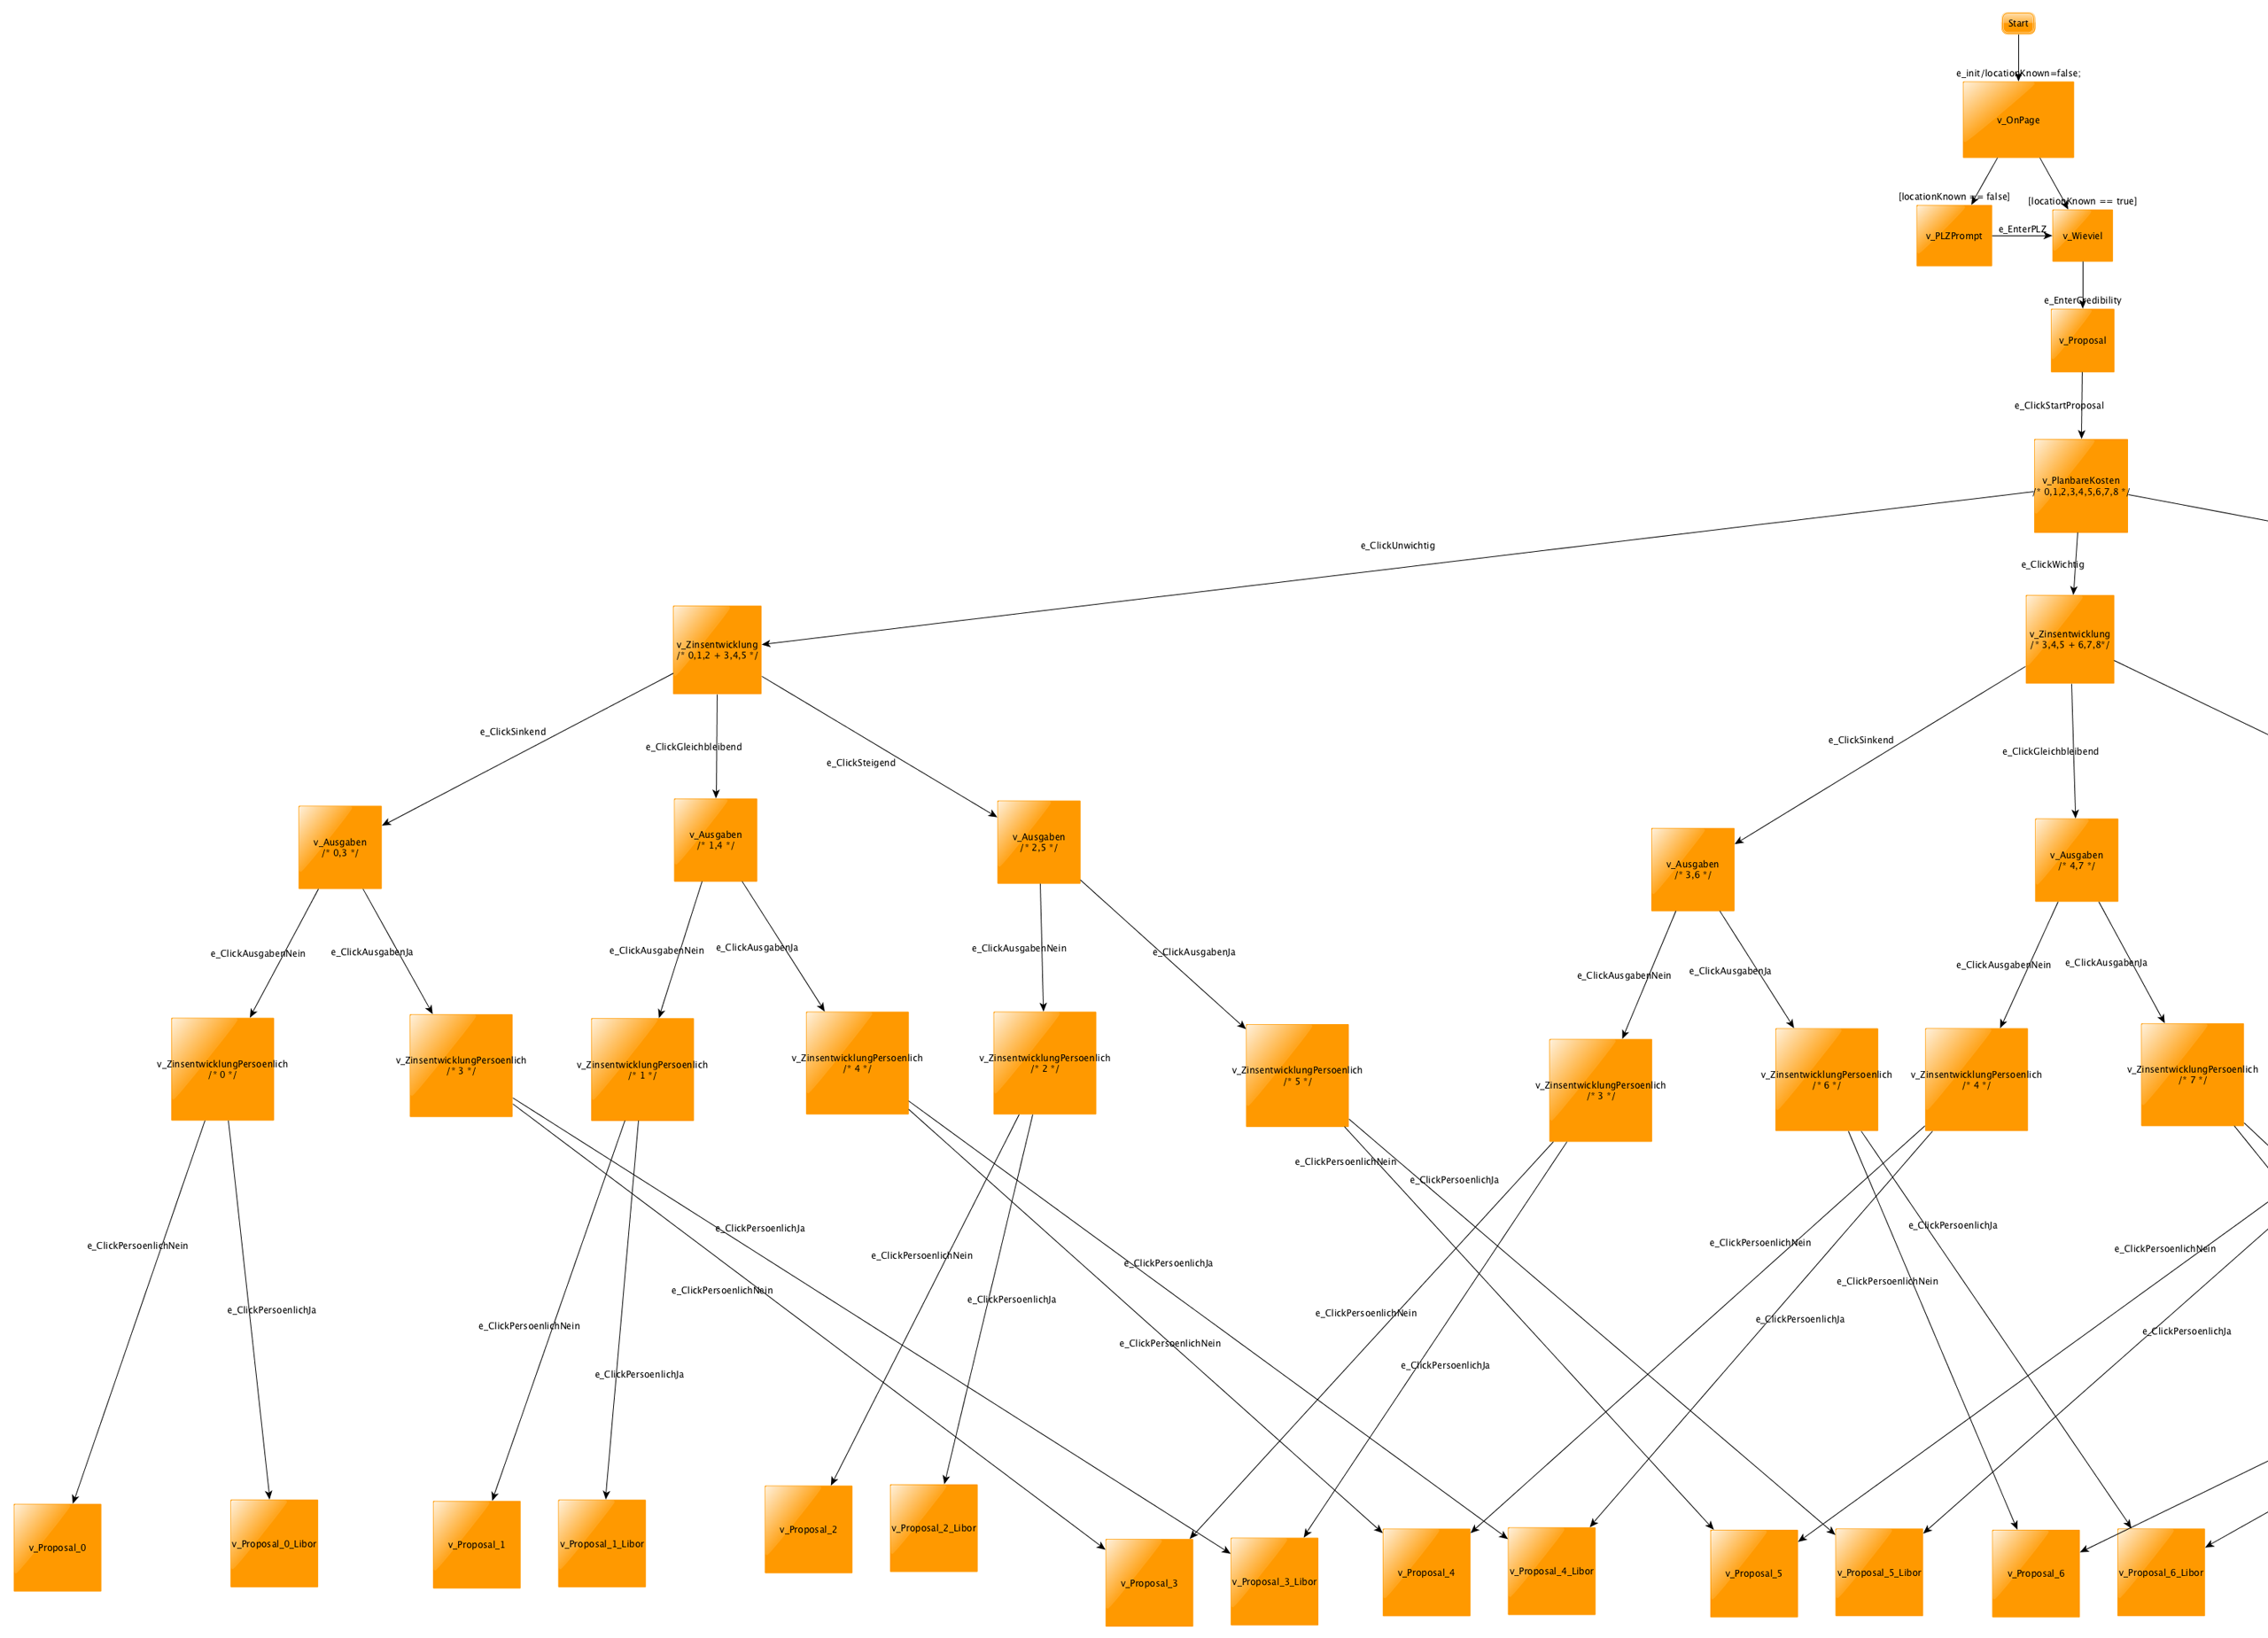
\includegraphics[width=1.3\textwidth]{figures/modell_logisch_left.png}
\caption{Ausgehend von der Logik-Modellierung wurde hier die Logik im Quellcode betrachtet. Linke Seite.}
\label{fig:modell_logisch}
\end{leftfullpage} 
\end{figure} 
\begin{figure}[p] 
\begin{fullpage}
\hspace*{-2cm}
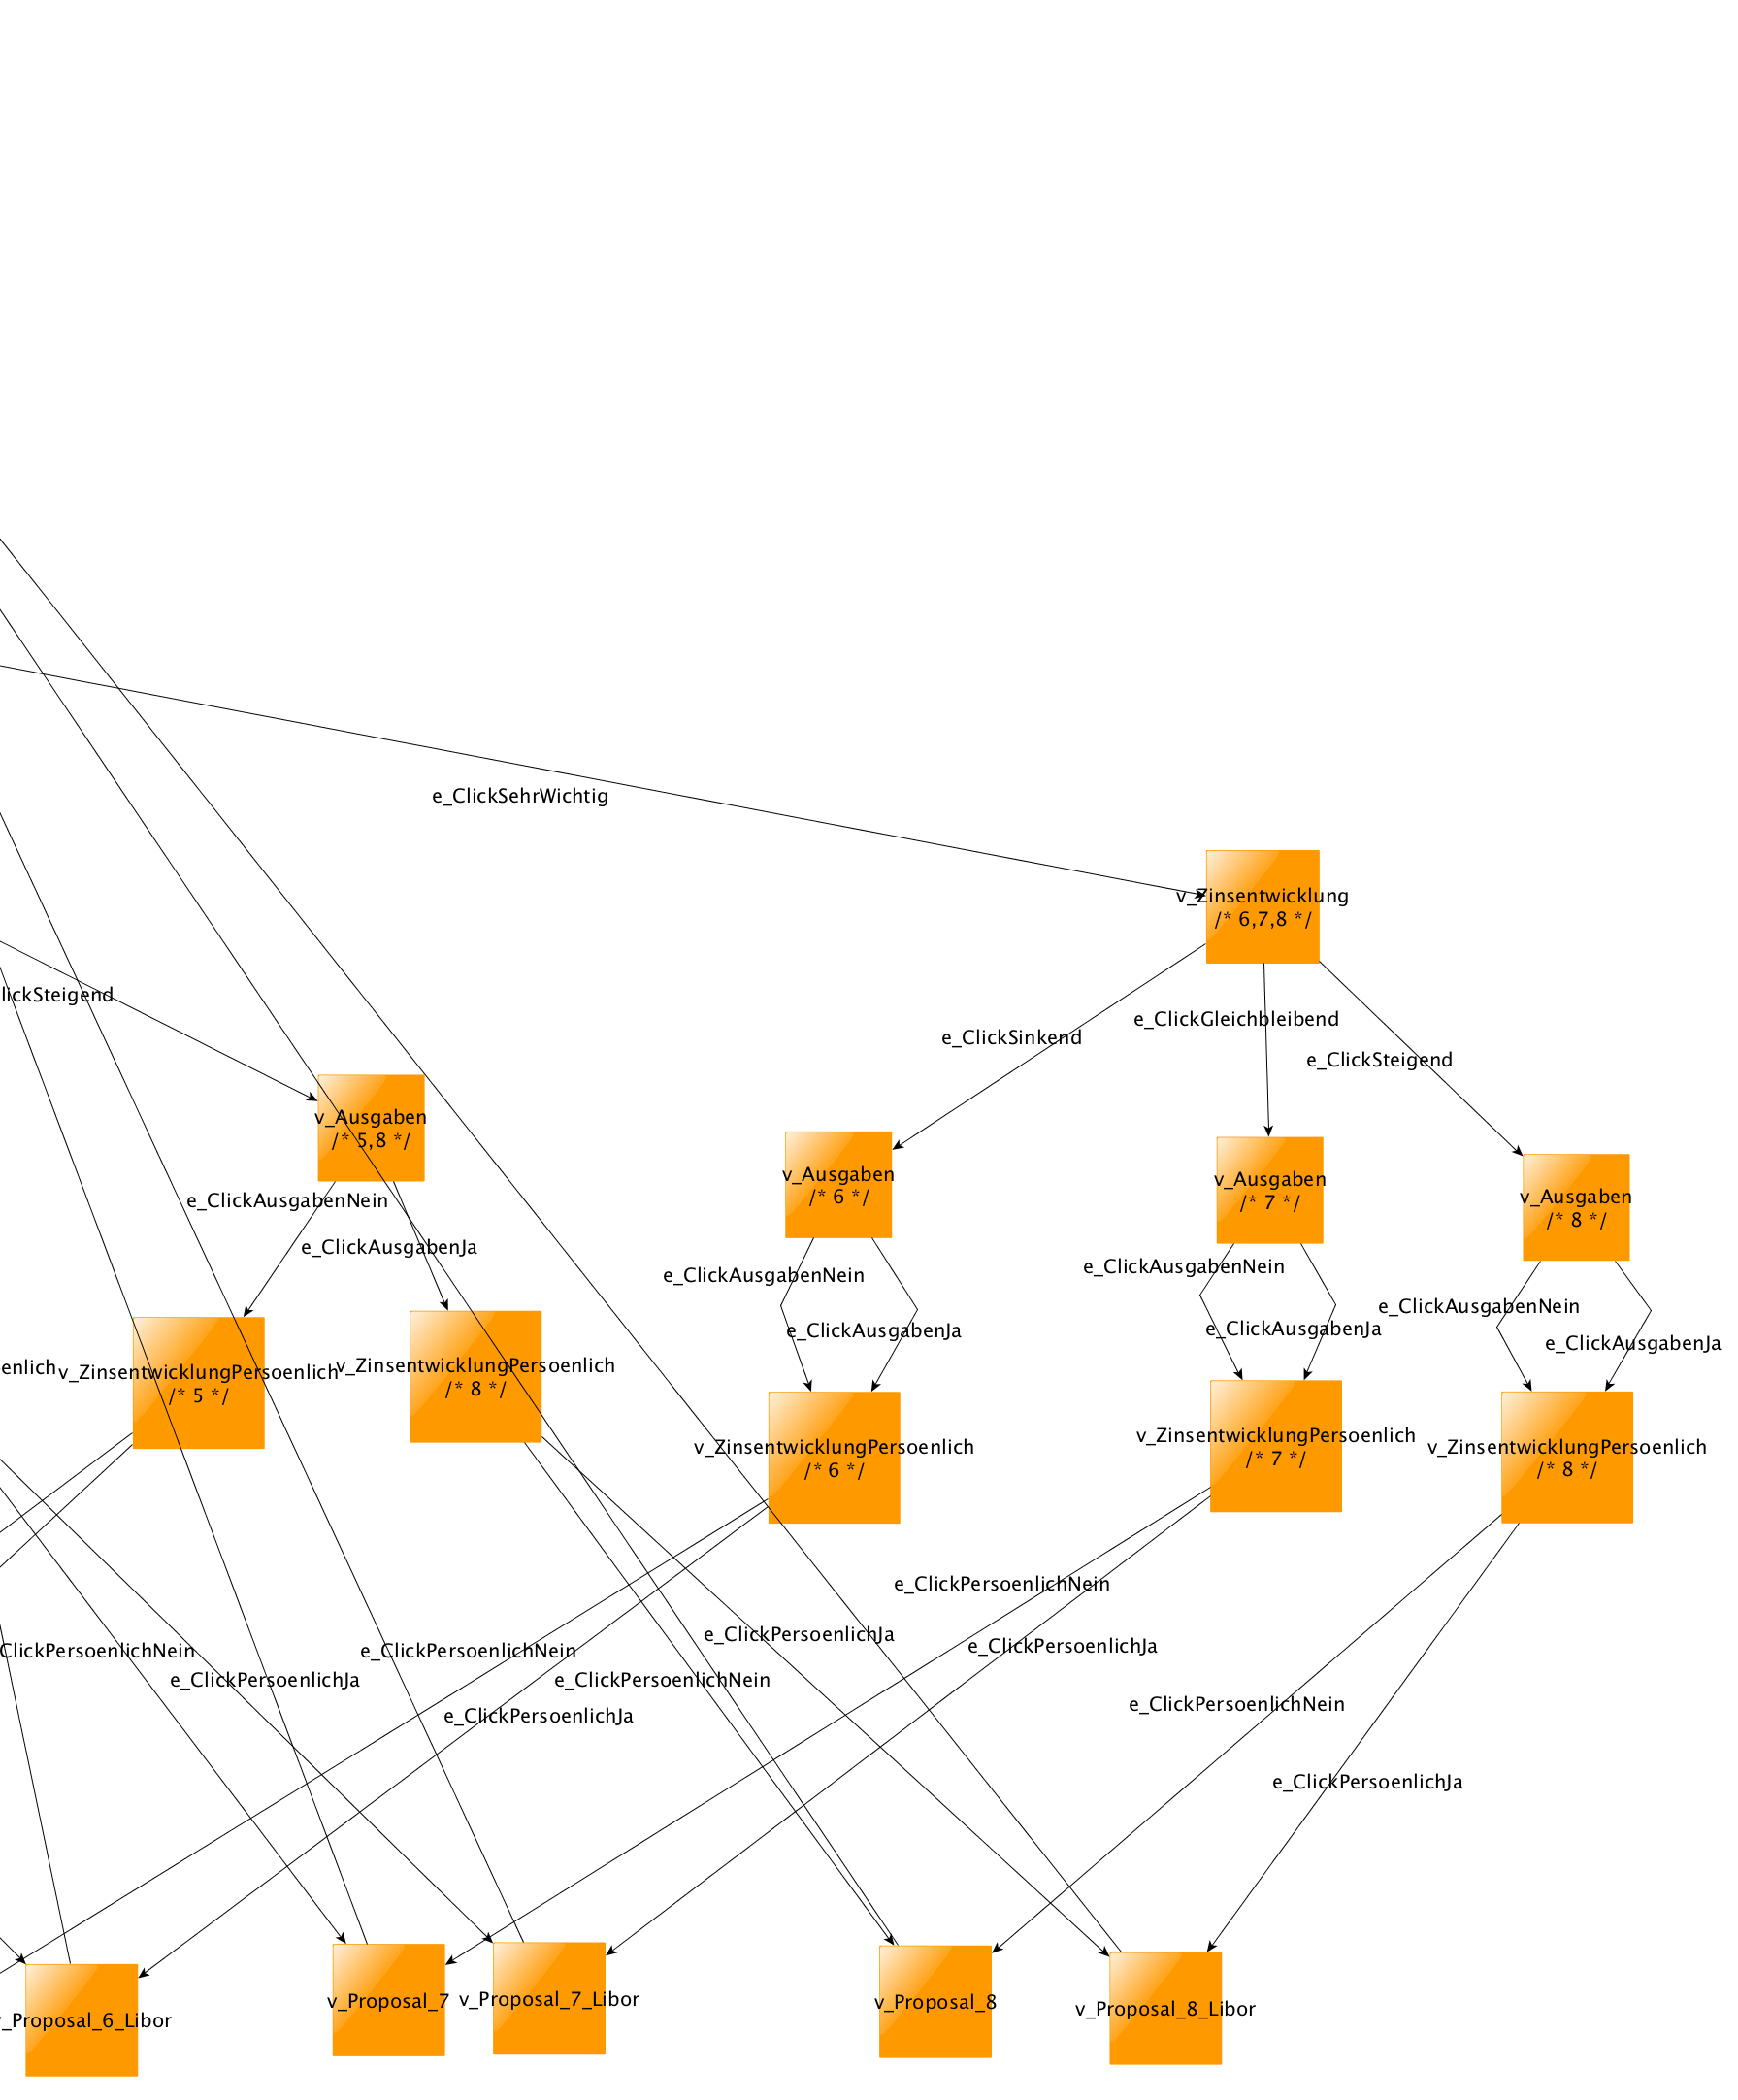
\includegraphics[width=1.2\textwidth]{figures/modell_logisch_right.png}
\caption{Ausgehend von der Logik-Modellierung wurde hier die Logik im Quellcode betrachtet. Rechte Seite.}
\end{fullpage} \end{figure} 

\subsubsection{Verbindung zwischen Modellen und \Gls{SUT}: Adapter-Code}
Die Verbindung zwischen dem abstrakten Testmodell und dem eigentlichen Testsystem herzustellen ist eine heikle Aufgabe mit jeder Teststrategie. Einerseits muss diese Verbindung überaus Zuverlässig sein, um kein Fehlverhalten bei der Ansteuerung des \Gls{SUT} zu provozieren. Andererseits darf es nicht zu aufwendig sein diesen Adapter-Code zu schreiben, damit wertvolle Ressourcen für das eigentliche Testen eingesetzt werden können. Graphwalker bietet bewusst keinerlei Funktionalität um die Zustände des Graphen auf das \Gls{SUT} abzubilden. Ein weiteres Werkzeug oder eine Bibliothek, die solche Funktionalität anbietet muss verwendet werden. Wie einleitend erwähnt eignet sich Graphwalker für das Testen auf beliebigen Ebenen, sofern die nötige Verbindung zur Steuerung des \Gls{SUT} hergestellt werden kann.\\
Für Tests auf Ebene der Benutzeroberfläche kann beispielsweise Selenium gewählt werden. Das Einfügen von Selenium Code erfolgt an genau definierten Stellen. Dazu wird das Graphwalker Modell im GraphML Format eingelesen. Graphwalker erzeugt daraufhin Java Interfaces, die der Testentwickler implementiert und an den annotierten Stellen mit Adapter-Code versieht.\\
Im Quellcodebeispiel \ref{lst:SeleniumImexPLZ} wird auf der Kante \texttt{e\_EnterPLZ}, welche darstellt, dass eine Maske mit der Aufforderung zur Eingabe der Postleitzahl angezeigt wird, eine Eingabe gemacht. Daraufhin wird das entsprechende Element angeklickt. Die Methode wurde vom Interface, welches Graphwalker automatisch anhand des Modells erzeugt hat, bereitgestellt. Der Testentwickler befüllt alle Knoten und Kanten, die nötig sind um den zu testenden Ablauf zu durchlaufen. 

\begin{lstlisting}[caption={Auf einer Kante wird mittels Selenium eine Eingabe und ein Klick durchgeführt.}, label=lst:SeleniumImexPLZ, float]
@Override
public void e_EnterPLZ() {
    WebElement searchBox = driver.findElement(By.className("dropdown-toggle"));
    searchBox.sendKeys("6900");
    driver.findElement(By.partialLinkText("Lugano")).click();
}
\end{lstlisting}

Aktionen wie Eingaben und Klicks werden typischerweise in den Kanten gespeichert. Knoten werden genutzt um Zustände zu überprüfen. Für solche Überprüfungen kann ein beliebiges Werkzeug verwendet werden. 
%Typischerweise befindet sich Code, der Aktionen wie Eingaben und Klicks ausführt, in den Kanten. Knoten, vor allem zum Schluss eines Ablaufs, werden dazu genutzt Zustände zu überprüfen. Auch für solche Überprüfungen kann ein beliebiges Werkzeug verwendet werden. 
Selenium bietet Möglichkeiten festzustellen, ob ein Element auf der aktuellen Eingabemaske sichtbar oder benutzbar ist. Das Quellcodebeispiel \ref{lst:SeleniumImexAssertion} zeigt wie im Knoten \texttt{e\_Proposal\_0} geprüft wird ob an einer bestimmten Stelle im HTML-Dokument der Text \texttt{Festhypothek} dargestellt wird. Um an diese Stelle im Dokument zu navigieren wird die \textit{XML Path Language}\footnote{Definition der XPath Version 1 des World Wide Web Consortium \url{http://www.w3.org/TR/xpath/}} verwendet.

\begin{lstlisting}[caption={Eine Assertion in Selenium auf einem Graphwalker Knoten}, label=lst:SeleniumImexAssertion, float]
@Override
public void v_Proposal_0() {
   //Beispielsweise
   Assert.assertTrue(driver.findElement(
	   By.xpath("//*[@id=\"maincontent\"/div/div/div[3]"))
	   .getText()
           .equals("Festhypothek"));
}
\end{lstlisting}

\subsubsection{Modellbasierte Tests auf niedrigeren Ebenen} Das Anwendungsbeispiel aus Abschnitt \ref{sec:results_modellierung} zeigt die Mächtigkeit von Graphwalker in Verbindung mit einem Framework für das GUI-Testing. Statt eines GUI-Testing-Frameworks können aber beliebige andere Frameworks als Adapter-Code verwendet werden. Damit wird das Testen auch auf Schnittstellen- und sogar Komponententestebene möglich. In Verbindung mit einer, darauf ausgerichteten, Testing API zum \Gls{SUT}, können aber genauso Tests der Businesslogik modelliert werden. Also eine Art Komponententest aus Sicht des Fachbereichs in Form eines Modells. Denkbar sind Abläufe wie das Laden eines Kunden, die Modifikation dessen Stammdaten und die abschließende Überprüfung, ob diese Modifikationen fehlerfrei abgelegt wurden. Die Modelle lassen eine unbegrenzte Komplexität zu. Seltene, lange aber geschäftskritische Workflows, lassen sich damit sehr gut darstellen.

%%%%%%%%%%%%%%%%%%%%%%%%%%%%%%%%%%%%%%%%%%%%%%%%%%%
\section{Stärken der Kombination von MBT und BDT}
\label{sec:mbt_bdt}
%%%%%%%%%%%%%%%%%%%%%%%%%%%%%%%%%%%%%%%%%%%%%%%%%%%%%%%

\todo[color=blue]{Schrift von yEd Graphen vergrößern}
Wie stark die Verwendung der drei Komponenten (FluentCoS, Testing API, MBT, siehe Abbildung \ref{fig:testarchitektur}) dieses Konzepts ineinander verzahnt werden muss fallabhängig entschieden werden. Denkbar ist einerseits ein vollständig isolierter Entwurf und Einsatz von \Gls{BDT} und \Gls{MBT}. Beide Sorten von Tests können unabhängig voneinander betrieben und gewartet werden. Außerdem können \Gls{BDT} und \Gls{MBT} auf den reichen Katalog der Testing API zugreifen. Somit lässt sich viel Wartungsaufwand für die Anpassung von Adapter-Code an einer Stelle, in der Testing API, konzentrieren.

\subsection{Parallelen zwischen MBT und BDT Testfällen}
\label{sec:mbt_bdt_parallelen}

Geht man einen Schritt weiter kann es Sinn machen, die strukturellen Ähnlichkeiten zwischen \Gls{BDT} und \Gls{MBT} Tests zu nutzen. Wie in Kapitel \ref{sec:bdd} erklärt, haben \Gls{BDT} Tests eine sehr einheitliche Form. Ausgehend von einem Startzustand, werden eine oder mehrere Aktionen durchgeführt, bis ein definierter Endzustand erreicht wird. Man stelle sich einen \Gls{BDT} Test als einfachen Pfad innerhalb eines Graphen vor. Tatsächlich könnte ein solcher Test in ein \Gls{MBT} Modell transformiert werden. Ein beträchtlicher Teil des Modells würde aber wahrscheinlich nur dazu dienen das \Gls{SUT} in den Startzustand zu führen. Im Gegensatz zum \Gls{BDT} Test, in dem dieser in der Regel sehr schnell aber dafür unpräziser definiert wird. Dieser Umstand wird in der Abbildung \ref{fig:mbt_bdt_given} veranschaulicht. Als Beispiel wird eine Internetbanking-Umgebung angenommen.

%Grafik: MBT vs BDT, langer schwanz bis startzustand erreicht. Ein pfad
\begin{figure} 
  \centering
     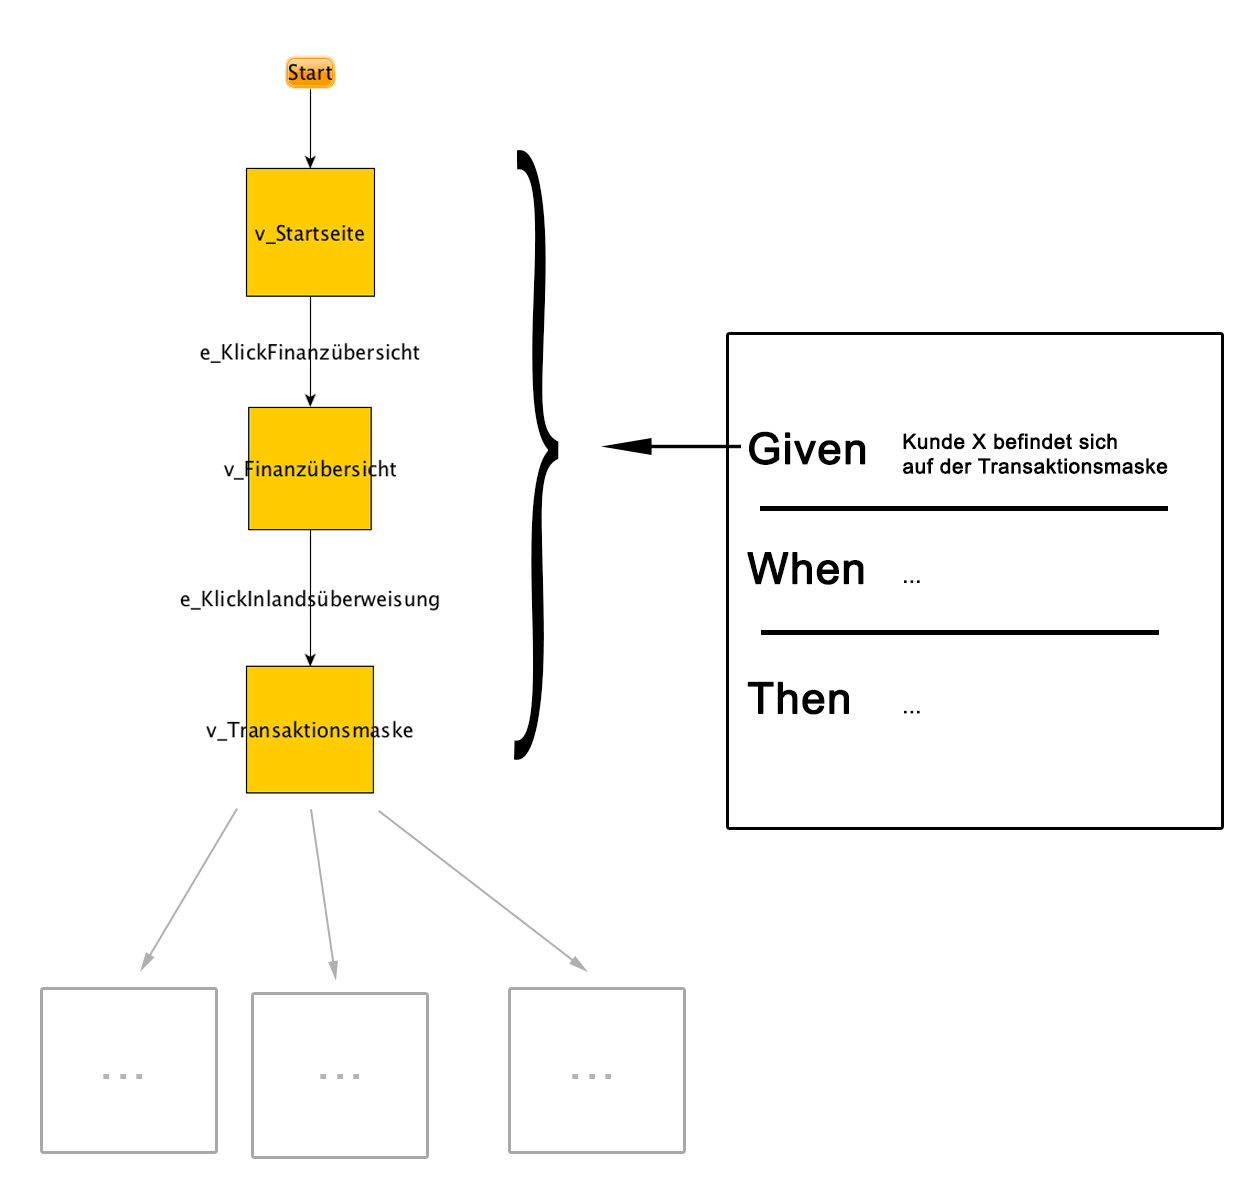
\includegraphics[width=0.8\textwidth]{figures/mbt_bdt_given.png}
  \caption{Transformation des \textit{Given} Teils eines BDD Tests in ein Modell}
  \label{fig:mbt_bdt_given}
\end{figure}

Nun würde die Aktion im \Gls{BDT} Test folgen. Diese wird, gerade in Cleartext \Gls{BDD} Spezifikation, oft nur kurz beschrieben (`Der Kunde macht eine Überweisung über 100 Euro an sein Sparkonto'). Dies hat zwei gravierende Nachteile: Einerseits ist abhängig vom Domänenwissen nicht klar was hier im Detail geschieht. Verschiedene Auffassungen können zu schwerwiegenden Fehlentscheidungen führen. Andererseits wird die Reproduktion durch die unpräzise Definition unter Umständen sehr schwierig. Ganz anders im Falle eines \Gls{MBT} Modells. Pro Kante wird eine, aus der Sicht des Benutzers, atomare Aktion ausgeführt. Auch wenn es Alternativen zur Ausführung einer Aktion gäbe, wäre dies im Modell sofort ersichtlich. Abbildung \ref{fig:mbt_bdt_when} zeigt eine solche Situation. Während im \Gls{BDT} Test nur eine abstrakte Beschreibung dessen vorkommt, was als Ergebnis dieser Aktion passiert, ist das Modell sehr ausdrucksstark. Im Beispiel führt ein Tastaturkürzel, ein Button und ein über Rechtsklick aufgerufenes Kontextmenü zur selben Maske.

%Grafik, WHEN teil, mehrere Alternativen wie EINE aktion ausgeführt werden kann
\begin{figure} 
  \centering
     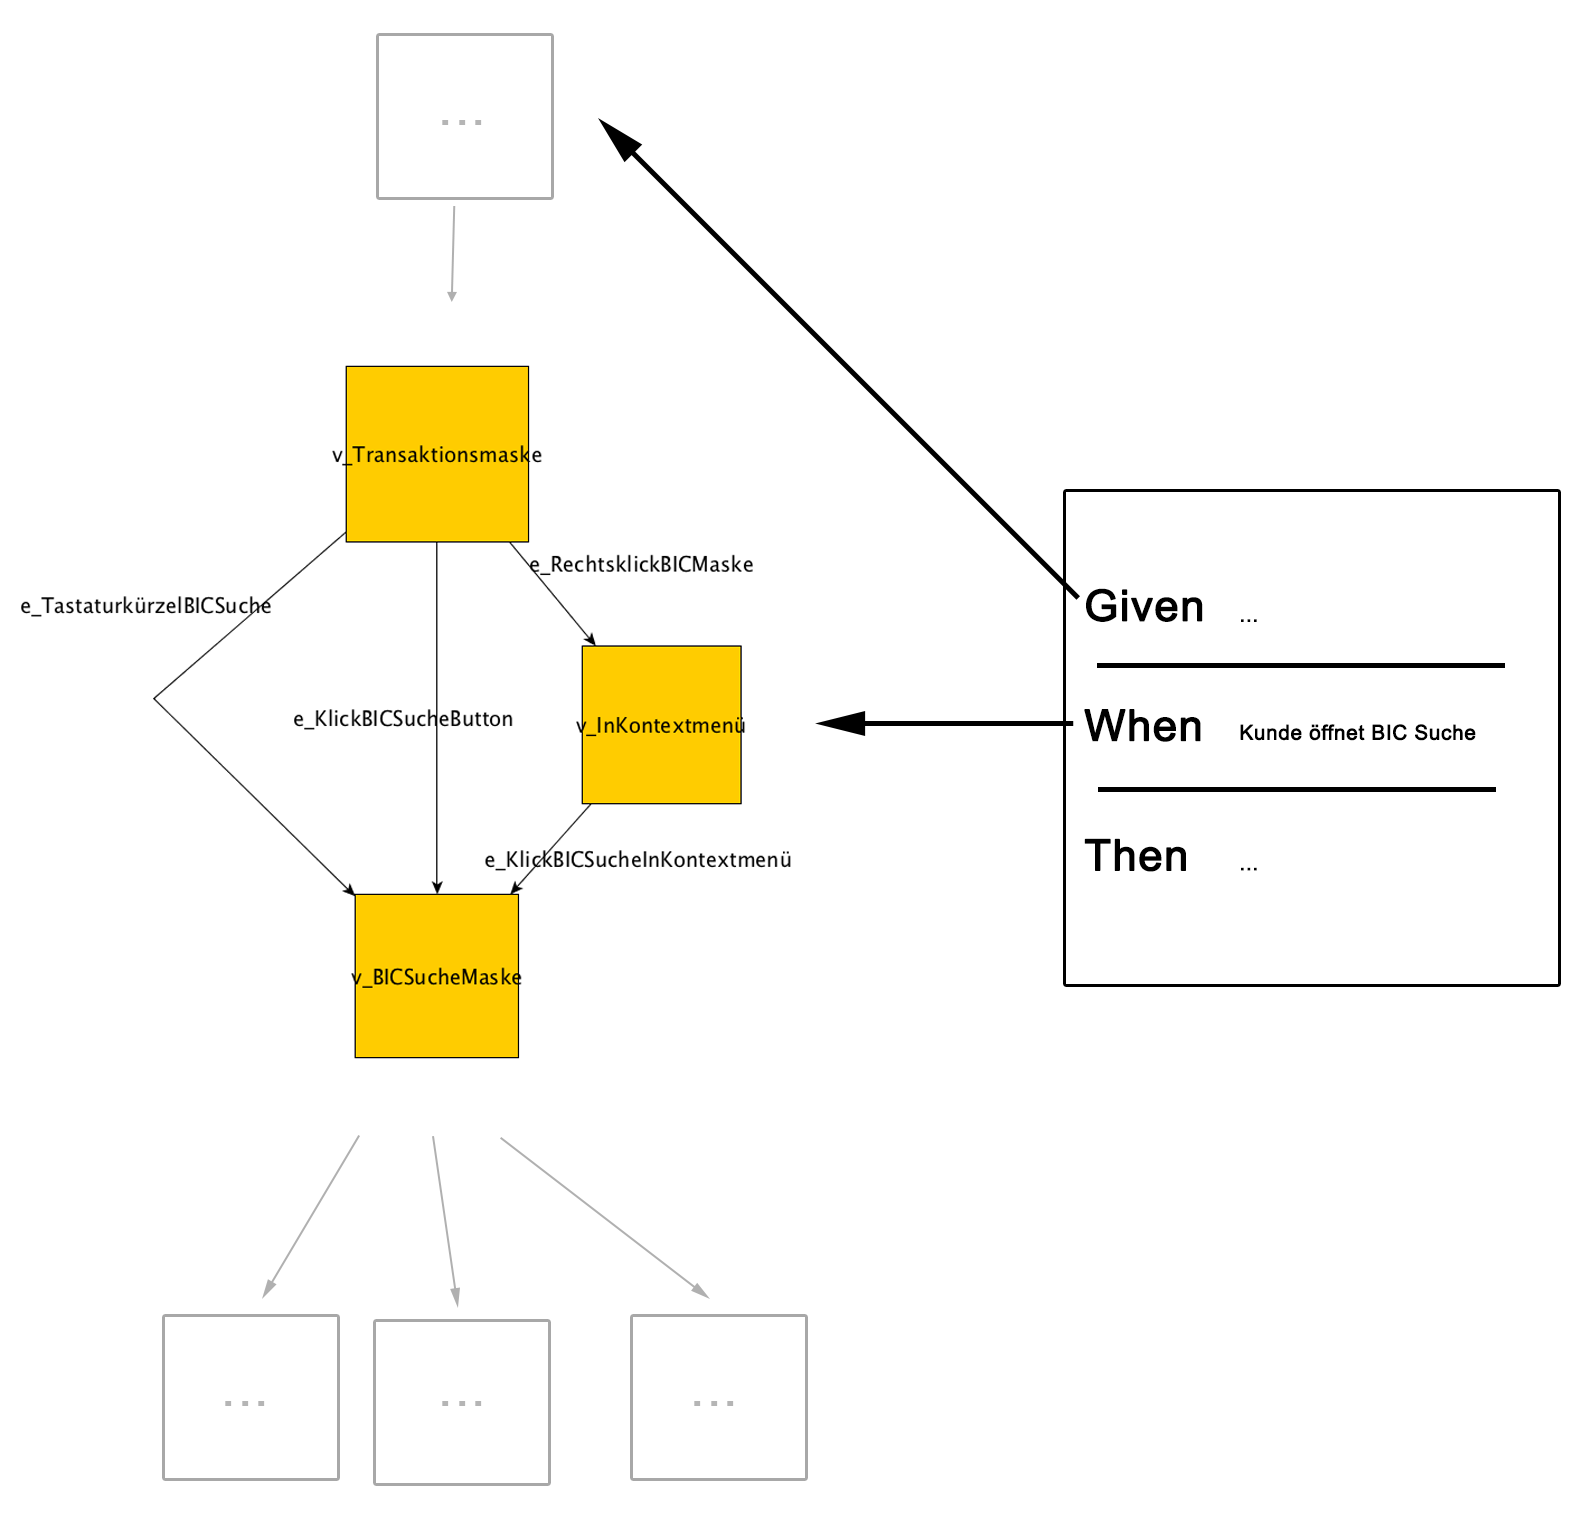
\includegraphics[width=1\textwidth]{figures/mbt_bdt_when.png}
  \caption{Ein Modell beschreibt Alternativen die im \textit{When} Teil des BDT Tests unerwähnt bleiben}
  \label{fig:mbt_bdt_when}
\end{figure}

Das endgültige Akzeptanzkriterium (\textit{then}) ist in \Gls{MBT} in einem ausreichend detaillierten Modell eine Überprüfung im Code. Auch im Beispiel \ref{fig:modell_logisch} aus Abschnitt \ref{sec:results_modellierung} ist im Modell nicht ersichtlich welche Überprüfungen in den Blattknoten genau gemacht werden. Hier zeigt sich wieder das Problem, dass sich Logik in der Implementierung des Modells versteckt. Abbildung \ref{fig:mbt_bdt_then} zeigt diesen Umstand grafisch. Im \Gls{BDT} Test kommen meist mehrere Kriterien zum Einsatz, die gleichzeitig erfüllt sein müssen. Da dieser sehr resultatsorientiert dargestellt und formuliert wird, ist sofort klar welche Eigenschaften des Systems im Endzustand geprüft werden. Es macht auch Sinn Überprüfungen außerhalb des gerade getesteten Kontexts zu machen. Im \Gls{BDT} Beispieltestfall in Abschnitt \ref{sec:bdt_bsp} wird genau das gemacht. Es findet eine lokale Überprüfung (`Die Karte sollte wieder ausgegeben werden' und `Eine erklaerende Fehlermeldung soll angezeigt werden') und eine Überprüfung des Zentralsystems statt (`Der Kontostand sollte unverändert bleiben). In Graphwalker würden solche Überprüfungen natürlich möglich sein. Es könnten dieselben Funktionen aus der Testing API verwendet werden, die auch im \Gls{BDT} Test vorkommen. Solche kontextübergreifenden Überprüfungen lassen sich in einem grafischen Modell aber nur schwer darstellen. Es wäre wiederum entscheidende Logik im Testcode verborgen. Codebeispiel \ref{lst:mbt_bdt_assertion} zeigt eine solche Einbettung von Überprüfungen in den Blattknoten aus Modell \ref{fig:mbt_bdt_then}.


\begin{lstlisting}[caption=Überprüfungen mittels Testing API in Blattknoten, label=lst:mbt_bdt_assertion]
/** Hier ist der THEN Teil des BDT Tests eingebettet */
@Override
public void v_TransaktionErfolgreich(){
  //Aufrufe an die Testing API innerhalb JUnit Assertions
  assert(TestingAPI.UI.transaktionErfolgreichPopUp());
  assert(TestingAPI.External.kontoBelastet(customerId, kontostandAlt-betrag));
  assert(TestingAPI.UI.anzeigeKontostand(kontostandAlt-betrag));
}
\end{lstlisting}


%Grafik komplett und Beschreibung wie Szenarien mehrere Zweige sein können usw.
\begin{figure} 
  \centering
     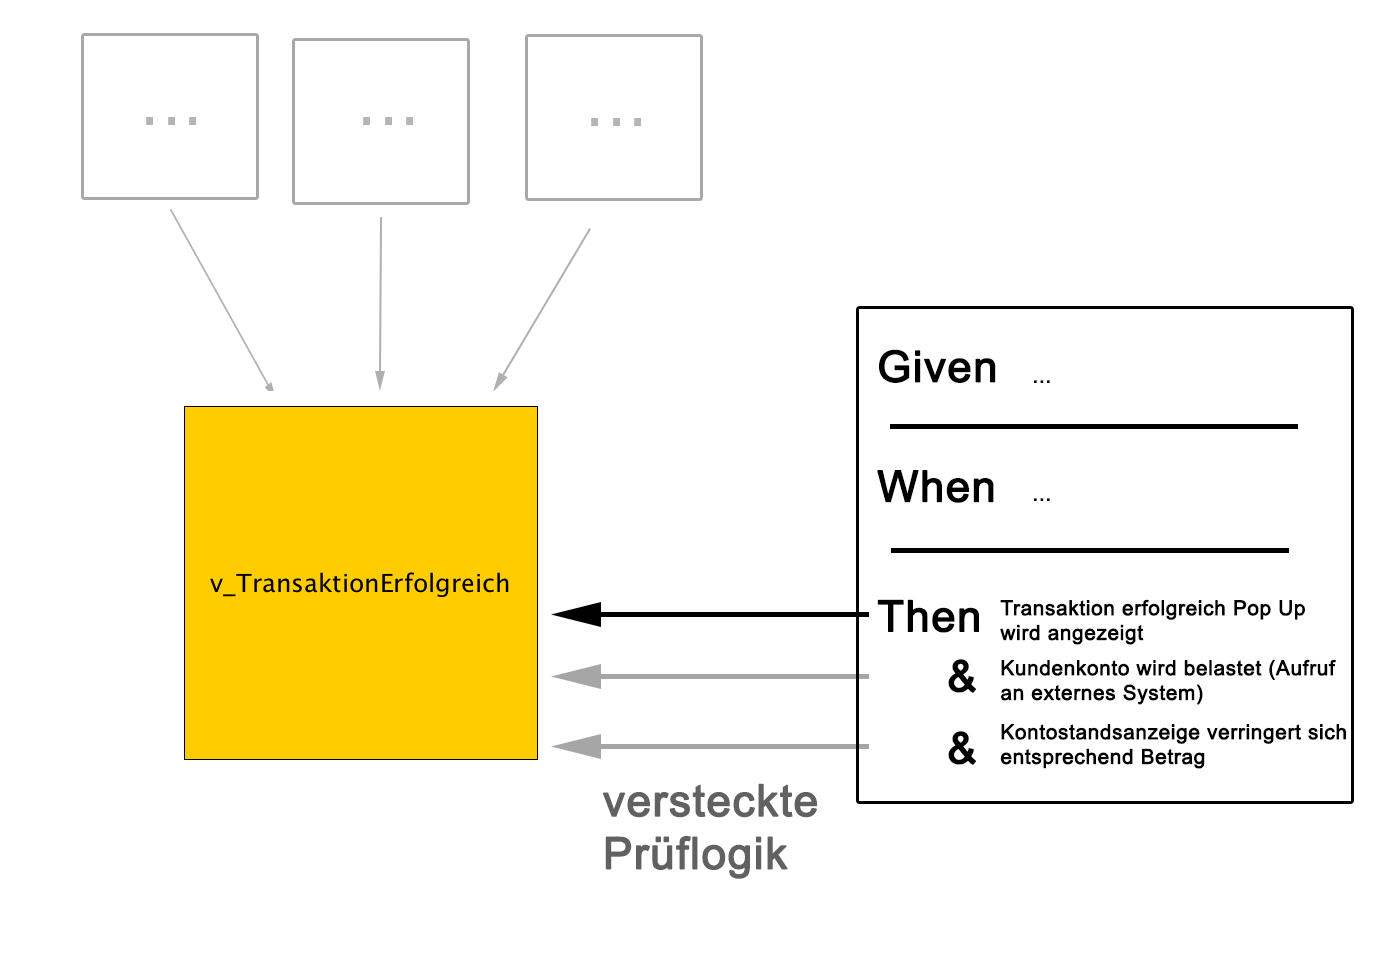
\includegraphics[width=1\textwidth]{figures/mbt_bdt_then.png}
  \caption{Die Überprüfungen bleiben im Code des Modells versteckt}
  \label{fig:mbt_bdt_then}
\end{figure}

\subsection{Konzept zur kombinierten Verwendung von BDT und MBT}
All die Erkenntnisse aus Abschnitt \ref{sec:mbt_bdt_parallelen} zusammengefasst, erlauben eine Kombination von \Gls{BDT} und \Gls{MBT}, die die Stärken beider Ansätze nutzt.\\
Auf oberster Ebene kann ein \Gls{BDT} Test, der aus $n$ Szenarien besteht, in ein Modell mit $n$ Startknoten oder Startpfaden dargestellt werden. Der Testentwickler wählt ein angemessenes Abstraktionsniveau und kann so die \textit{Given} Teile der einzelnen Szenarien, inklusive dem Kontext aus der \Gls{BDT} Erzählung, modellieren. Zu sehen sind diese Parallelen in der Abbildung \ref{fig:mbt_bdt_gesamt}. In diesem Beispiel unterscheiden sich die Szenarien anhand der Art des Kunden der das \Gls{SUT} bedient. Dies kann als gegebene Konfiguration gesehen werden und somit als einzelner Knoten modelliert werden (so wie in der Abbildung \ref{fig:mbt_bdt_then}). Andererseits kann dieser Schritt auch ausmodelliert werden. Technisch ist diese Unterscheidung mit Graphwalker sehr elegant lösbar. Wie im Abschnitt \ref{sec:graphwalker_funktionsweise} \nameref{sec:graphwalker_funktionsweise} erklärt, werden hier \textit{Guards} genutz. Alle drei Szenarienknoten sind valide Einstiegspunkte für die Traversierung des Modells. Abhängig von welchem Knoten die Traversierung gestartet wird, wird eine Guard Variable auf wahr gesetzt. Beginnt Graphwalker die Traversierung über den Knoten \texttt{v\_PrivatkundeVermögend} so wird die Variable \texttt{pkv} auf \texttt{true} gesetzt. Diese kann als globale Variable gesehen werden, die zu einem späteren Zeitpunkt während der Traversierung abgefragt werden kann.\\
Wenn sich die \textit{When} Schritte in den Szenarien unterscheiden, können diese vollständig dargestellt werden. Im Beispiel haben alle drei Szenarien diesen Teil gemeinsam und sind deshalb gleichfarbig. Im Hintergrund sind dies Codestücke die nicht mehrfach gewartet werden müssen. Auch wenn sich die Szenarien in diesem Teil unterscheiden kann hier die volle Stärke von \Gls{MBT} ausgenutzt werden und jeder Alternativpfad modelliert werden (so wie im vorangegangen Beispiel \ref{fig:mbt_bdt_when}).\\
Jedes Szenario kann nun seinen gänzlich eigenen Pfad einschlagen oder auch mit mehreren anderen Szenarien Pfade teilen. In den Blattknoten wird die erwähnte Expressivität des \Gls{BDT} \textit{Then} Teils genutzt. Da \Gls{BDT} Tests im Hintergrund als Adapter-Code die Testing API (siehe Abschnitt \ref{sec:testing_api}) verwenden, können diese Codefragmente problemlos in die Graphwalker Methoden eingebettet werden.\\
Es ist empfehlenswert eine grafische oder dokumentarische Verbindung zwischen den so kombinierten Testfällen im Projekt zu halten. Gerade die Überprüfungen in den Blattknoten, in denen \Gls{BDT} Überprüfungen eingebettet sind, sind im Detail sehr interessant.

\begin{figure}
\hspace*{-2cm}
  \centering
     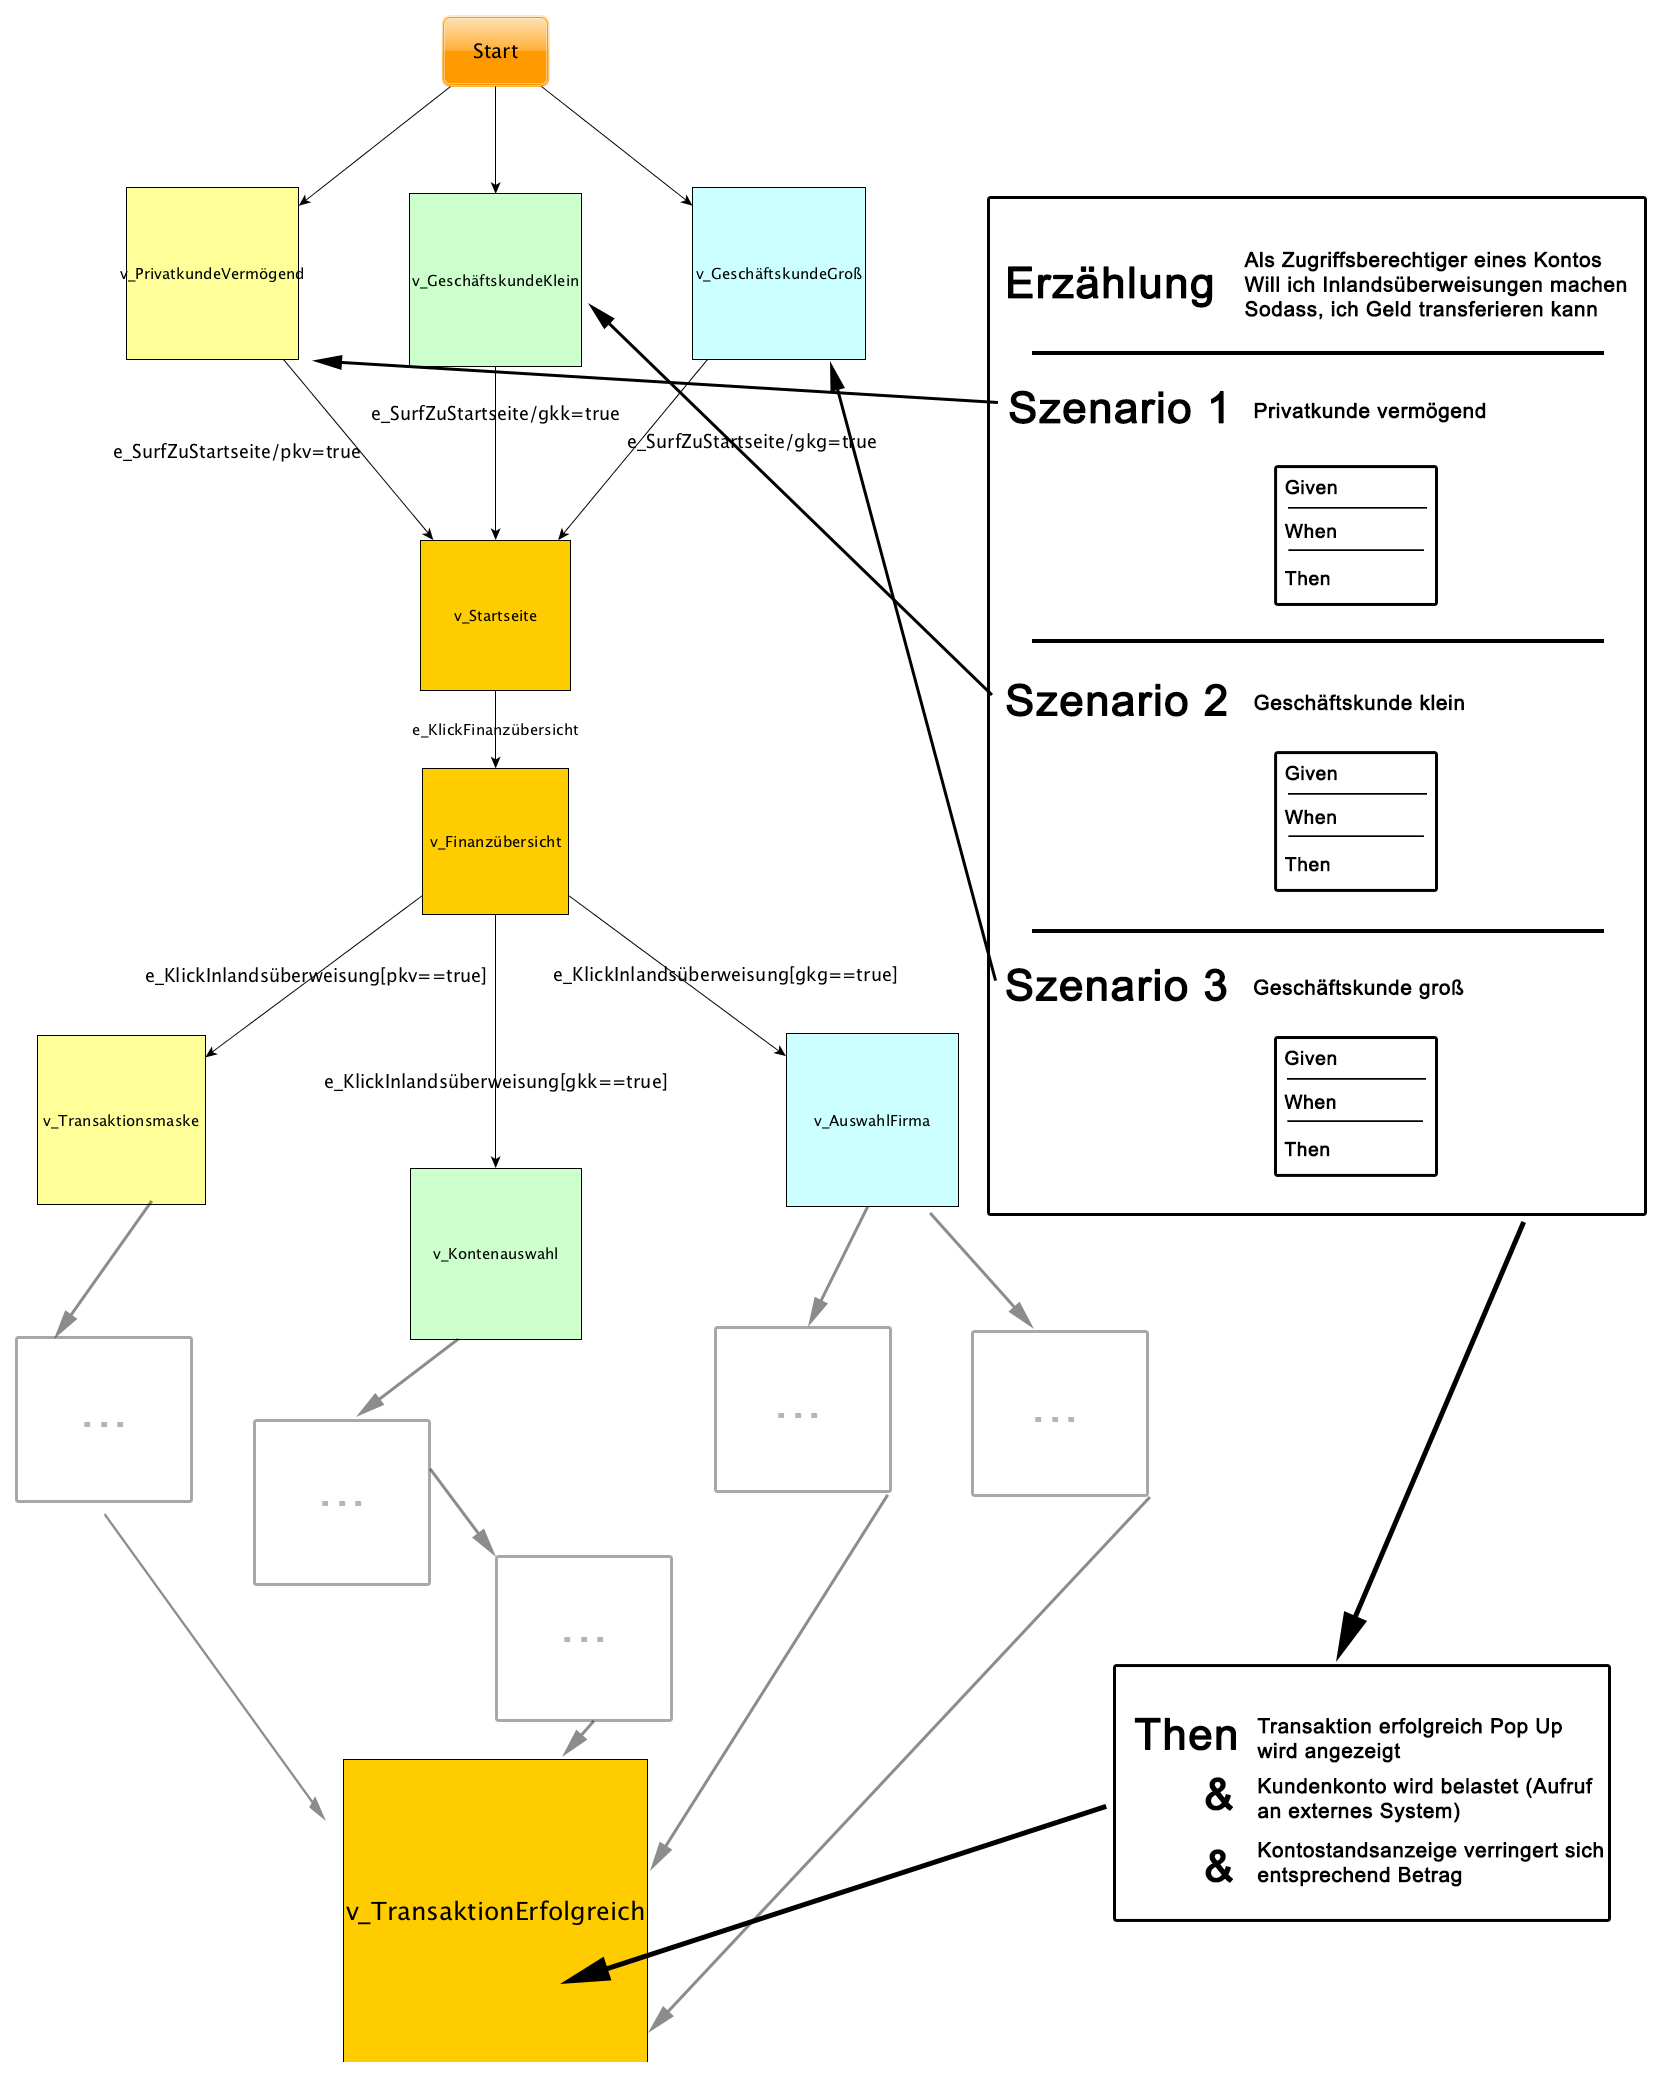
\includegraphics[width=1.25\textwidth]{figures/mbt_bdt_gesamt.png}
  \caption{BDT Szenarien können im Modell explizit dargestellt werden}
  \label{fig:mbt_bdt_gesamt}
\end{figure}


\section{Zugewinne durch die vorgestellte Teststrategie}
Gerade für die agile Entwicklung ist die Kombination von BDD und \Gls{MBT} wie maßgeschneidert. Agile Entwicklung bedeutet unter anderem viel Kontakt mit dem Kunden und damit auch die Notwendigkeit der Auseinandersetzung mit Spezifikationsänderungen und Feedback. \Gls{COS}-artige Definitionen kommen in vielen Softwareprojekten bereits zum Einsatz und sind daher sowohl dem fachlichen als auch dem technischen Personal bekannt. Der Schritt von \Gls{COS}-Tabellen zu \Gls{BDT}-Testfällen, egal welches Framework dazu benutzt wird, ist unkompliziert. Wenn der Einsatz von \Gls{BDT}-Tests sorgfältig und gut koordiniert umgesetzt wird, ist die damit einhergehende Versionierung der \Gls{COS} ein wertvoller Nebeneffekt, der die Organisation des Softwareprojekts vereinfacht.\\
Eine ähnliche Kombination von Methoden schlägt auch \citeauthor{binder_model-based_2014} vor \cite{binder_model-based_2014}. Er warnt aber davor, dass \Gls{BDT} nur einen kleinen Teil des \textit{happy-path} abdecken. Soll heißen, dass das System mittels \Gls{COS} nur auf sehr wenigen Pfaden getestet wird. Außerdem wächst die Anzahl der zu wartenden \Gls{BDD}-Spezifikationen mit der Größe der Code-Basis. Meist hat dies zur Folge, dass ältere Spezifikationen in Vergessenheit geraten und nicht mehr in die Regressionstests miteinbezogen werden. Um zweiterem Nachteil entgegenzuwirken müssen \Gls{BDD}-Spezifikationen sehr sorgfältig und mit Hinblick auf die Programmlogik entworfen werden. Außerdem muss die Versionierung Teamübergreifend nahtlos funktionieren.\\
Aus Kundensicht sind \Gls{COS} oft notwendig, da sie kurz und bündig vertragliche Abkommen darstellen können. Auch wenn der Kunde beim Abnahmetest auf \Gls{COS} Spezifikationen besteht, muss das System durch breitere Maßnahmen regressiv getestet werden. Hier ergänzen modellbasierte Tests die Qualitätssicherungsmaßnahmen. Ein \Gls{COS} kann als einzelner Pfad in einem Modell gesehen werden. Der modellbasierte Test prüft dann, mit variablem Grad an Prüflogik, alle anderen Pfade. Diese Vorgehensweise schafft eine weitere Schicht an Sicherheit und lässt sich gut in bestehende Projekt- und Softwarestrukturen integrieren. Durch die Nutzung einer durchdachten Testing API (wie in Abschnitt \ref{sec:testing_api} beschrieben) können Wartungsaufwände minimiert werden, indem nur eine Codebasis für Adapter-Code besteht. Die Testing API stellt außerdem eine zukunftssichere Barriere vor Änderungen auf Seiten des Testwerkzeuges dar. Dieses kann ausgetauscht werden ohne die Aufwände für die Anbindung des \Gls{SUT} zunichte zu machen.\\
Die in Abschnitt \ref{sec:mbt_bdt} vorgeschlagene kombinierte Verwendung von \Gls{BDT} \todo{wieso wird BDT abgekürzt und MBT ausgeschrieben? BEI MIR WIRD IM KOMPILIERTEN TEXT BEIDES ABGEKÜRZT} und \Gls{MBT} lässt das Projekt von den Stärken beider Ansätze profitieren. \Gls{BDT} und \Gls{MBT} lassen sich sehr flexibel miteinander verschmelzen und sowohl den technischen als auch den organisatorisch geschäftlichen Prozessen anpassen. Das \Gls{SUT} kann damit systematischer und flächendeckender getestet werden ohne signifankte Mehraufwände in Kauf nehmen zu müssen.











